% Chapter 7: Frontend Architecture
\chapter{Frontend Architecture} \label{ch:frontend-architecture}

\section{Overview of UI Architecture}

The Ollama UI application follows a modern, component-based architecture built with React and leveraging the latest frontend development practices. The application is designed to provide a responsive, intuitive interface for interacting with AI models through the Ollama backend.

\subsection{React Application Structure}

The application is built using React 19.0.0 and structured as a Single Page Application (SPA) with client-side routing. The project uses Vite 6.2.0 as the build tool and development server, providing fast refresh capabilities and optimized production builds.

The overall application structure follows these key organizational principles:

\begin{itemize}
  \item \textbf{Feature-based organization} - Code is organized by feature rather than by type
  \item \textbf{Modular components} - Components are designed to be reusable and focused on specific responsibilities
  \item \textbf{Clear separation of concerns} - UI components are separated from business logic and state management
  \item \textbf{Progressive enhancement} - The application is designed to work well across different devices and capabilities
\end{itemize}

The application's build process is configured for both development and production environments, with specific optimizations for deployment to GitHub Pages.

\subsection{Component Organization}

The UI components are organized into a clear hierarchy that promotes reusability and maintainability:

\begin{sidewaysfigure}[p]
    \centering
    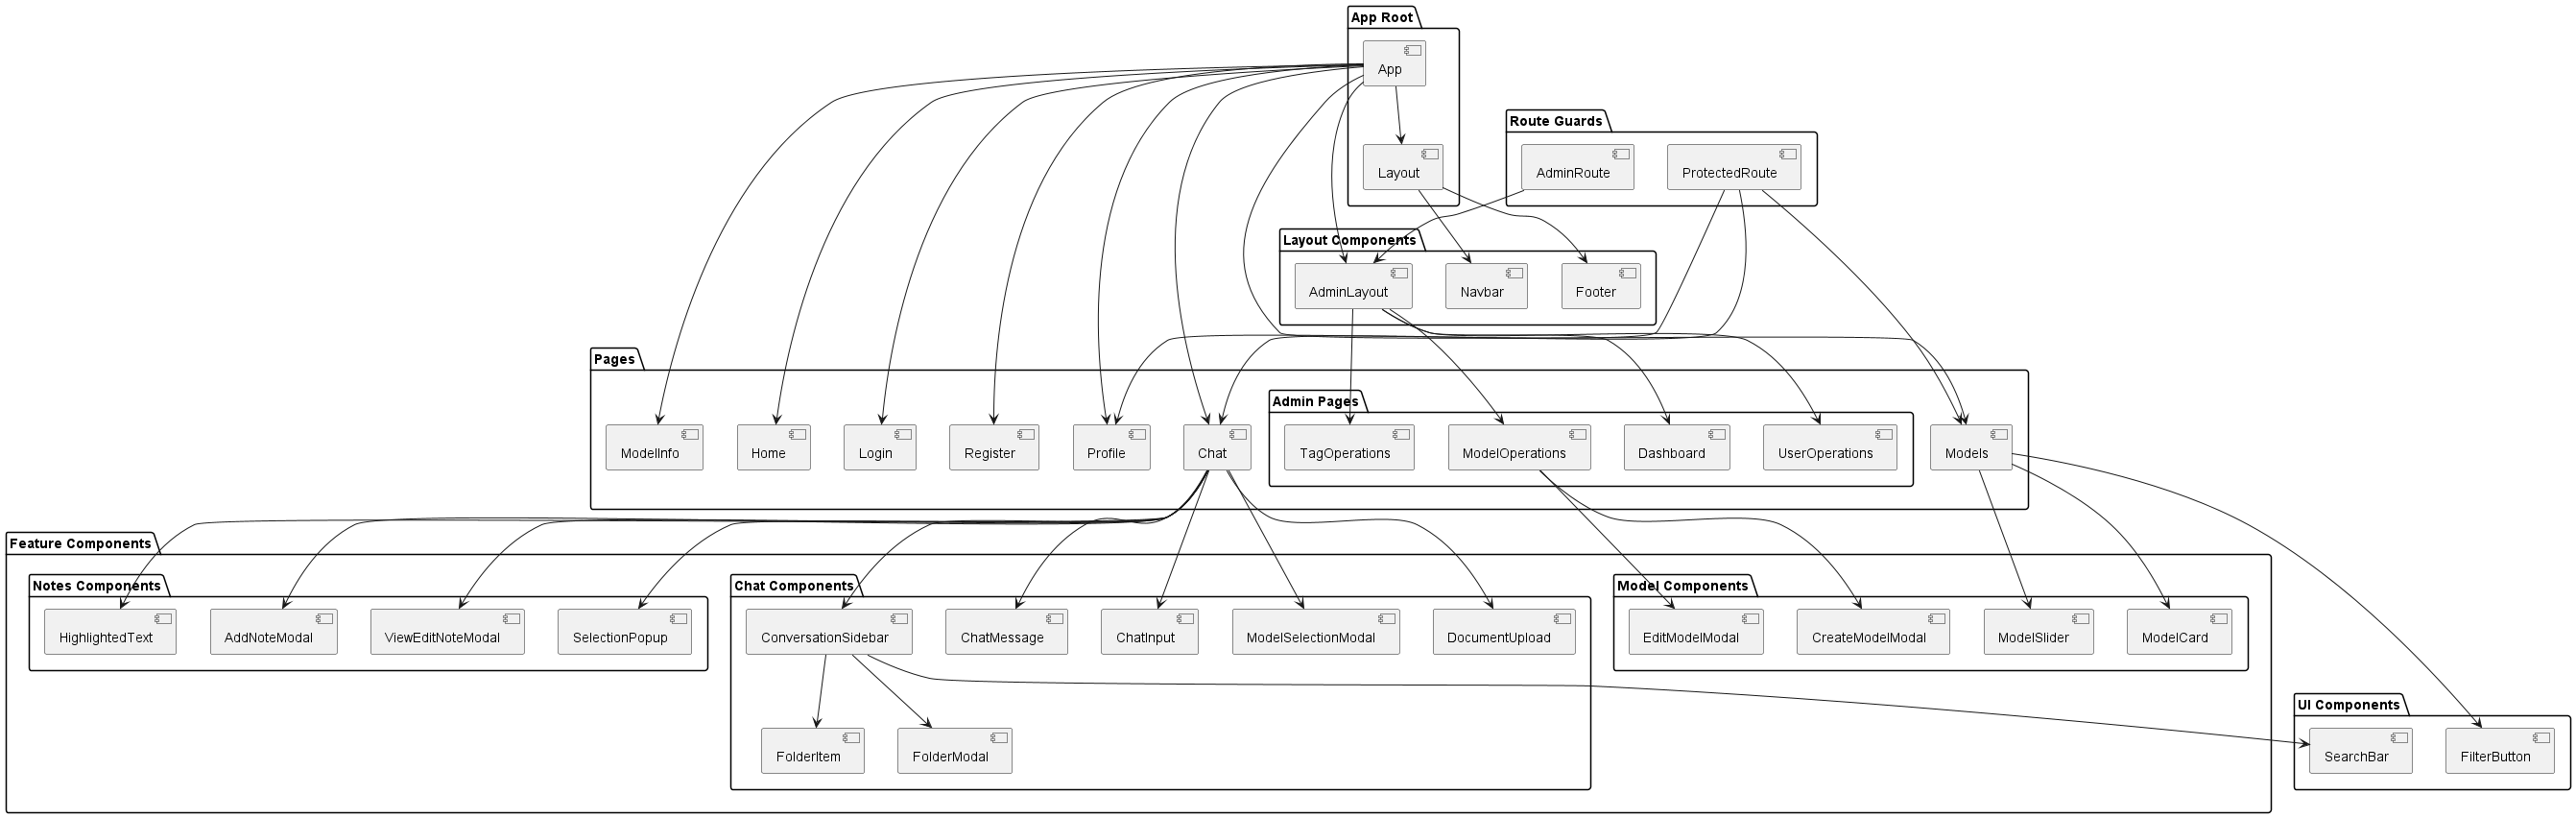
\includegraphics[width=\textwidth]{./Chapter07/figures/component_hierarchy.PDF}
    \caption{Component Hierarchy and Organization}
    \label{fig:component-hierarchy}
\end{sidewaysfigure}
\clearpage

The component organization follows these patterns:

\begin{itemize}
  \item \textbf{Page Components} - Top-level components rendered by routes (Home, Chat, Models, Profile)
  \item \textbf{Layout Components} - Provide consistent page structure (Layout, Sidebar, Header)
  \item \textbf{Feature Components} - Domain-specific components grouped by feature area (chat/, models/, admin/)
  \item \textbf{UI Components} - Reusable, generic UI elements (buttons, cards, modals, form elements)
  \item \textbf{Context Providers} - Wrap the application to provide global state (AuthProvider, ConversationProvider)
\end{itemize}

This organization ensures that components are easy to locate, maintain, and reuse throughout the application.

\subsection{State Management Approach}

Rather than using a state management library like Redux, the Ollama UI application leverages React's built-in Context API for global state management. This approach provides several benefits:

\begin{itemize}
  \item Simplified state management without additional dependencies
  \item Context providers organized by domain (Auth, Conversation)
  \item Custom hooks that expose context functionality to components
  \item Local component state for UI-specific concerns
\end{itemize}

\begin{figure}[p]
    \centering
    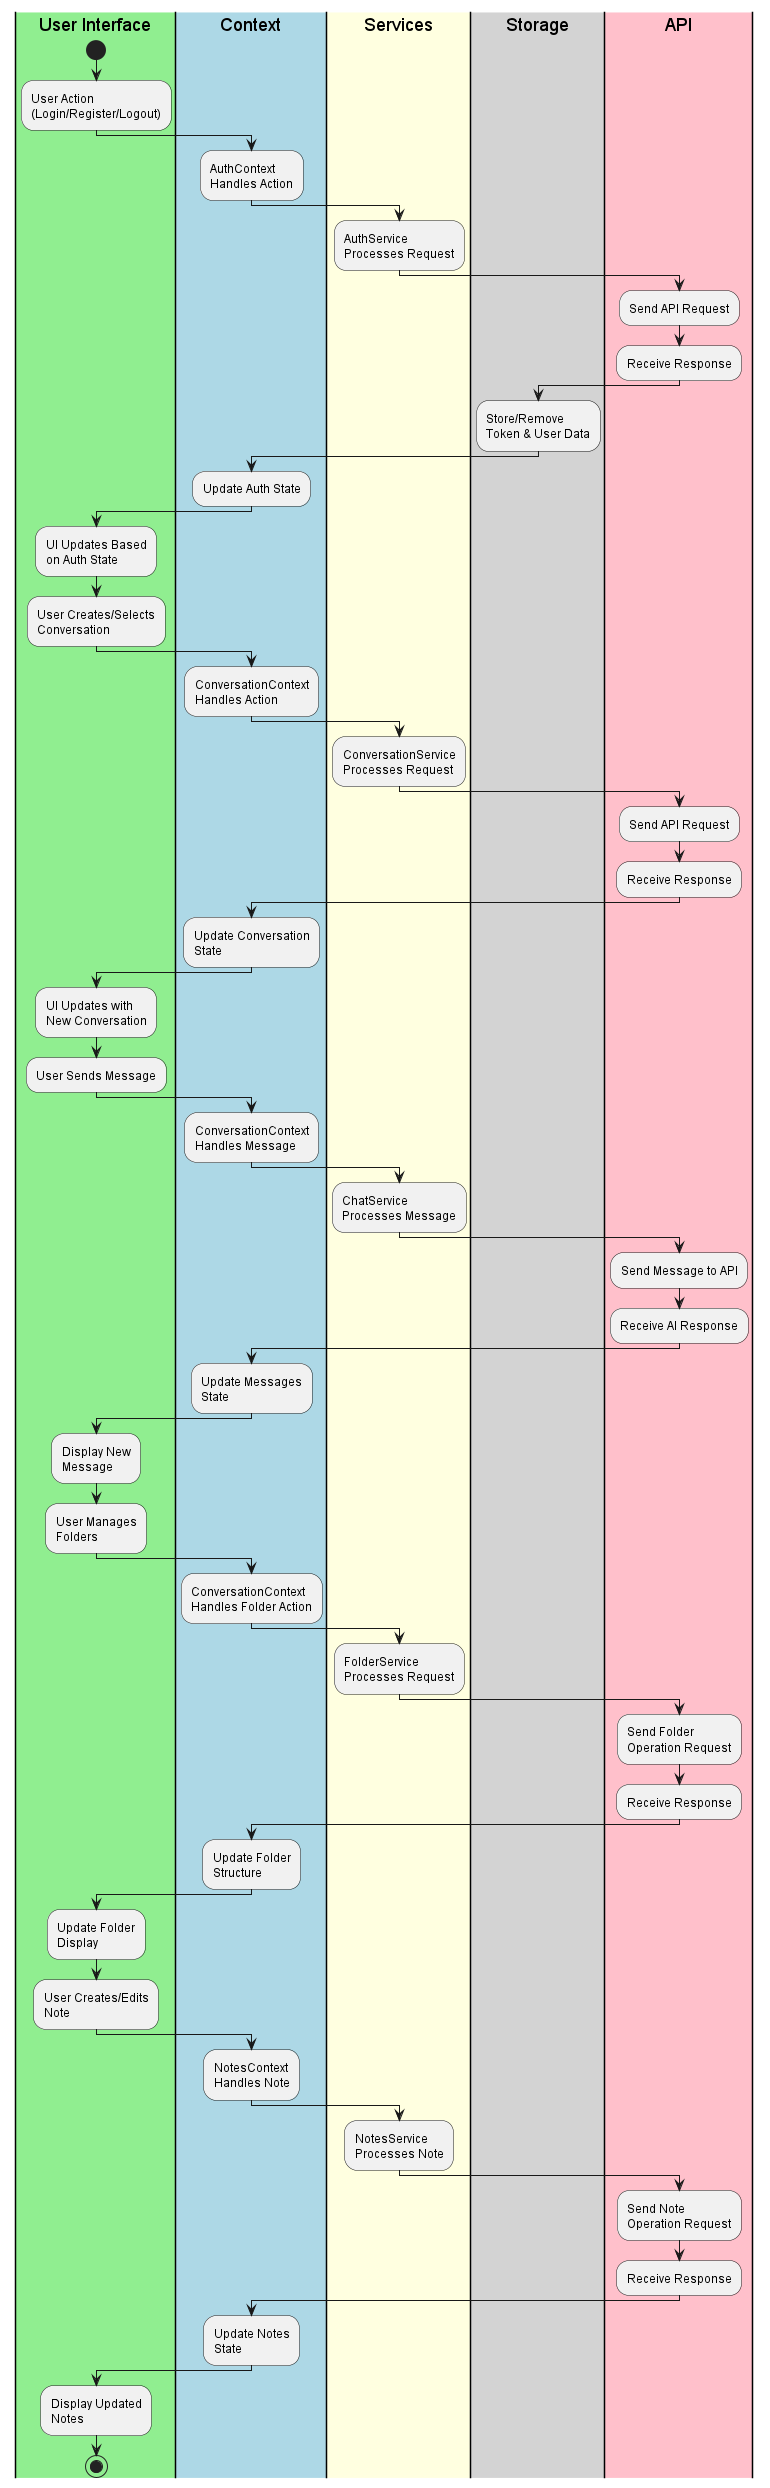
\includegraphics[width=\textwidth,height=\textheight,keepaspectratio]{./Chapter07/figures/state_management_flow.PDF}
    \caption{State Management Flow Between Components}
    \label{fig:state-management-flow}
\end{figure}
\clearpage

The application also uses TanStack React Query 5.80.7 for data fetching and caching, providing efficient API communication and state synchronization.

\subsection{Routing Implementation}

Client-side routing is implemented using React Router 7.2.0, which provides a declarative approach to navigation within the single-page application. The routing system includes:

\begin{itemize}
  \item Declarative route definitions
  \item Nested routes for consistent layouts
  \item Protected routes for authenticated content
  \item Role-based route protection
  \item Dynamic route parameters for entity-specific views
\end{itemize}

The router is configured with a base URL that supports deployment to GitHub Pages while maintaining proper navigation.

\section{Core UI Components}

The Ollama UI application is built using a collection of reusable core components that provide consistent functionality and appearance throughout the application. These components form the building blocks for more complex feature-specific interfaces.

\begin{sidewaysfigure}[p]
    \centering
    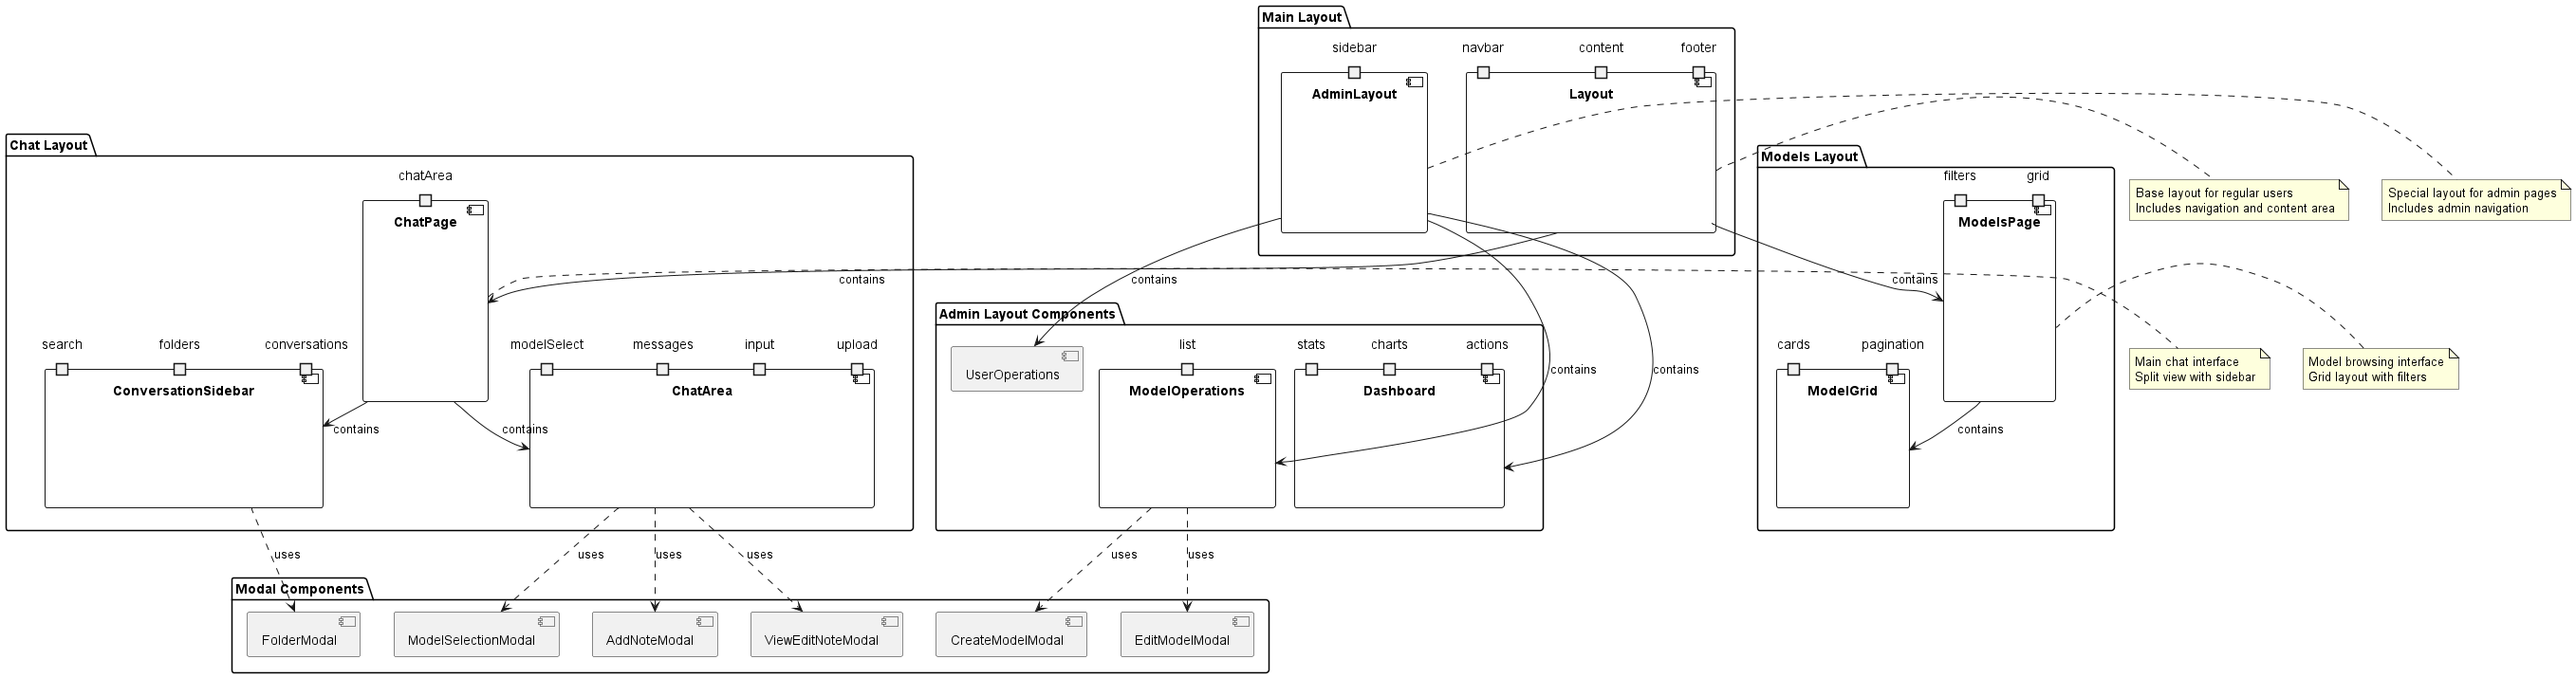
\includegraphics[width=\textwidth]{./Chapter07/figures/ui_layout_structure.PDF}
    \caption{UI Layout Structure and Responsive Breakpoints}
    \label{fig:ui-layout-structure}
\end{sidewaysfigure}
\clearpage

\subsection{Layout Components}

The application uses a consistent layout structure across different pages, implemented through reusable layout components:

\begin{itemize}
  \item \textbf{Layout} - The main layout component that wraps the entire application interface
  \item \textbf{Sidebar} - Navigation sidebar that provides access to key application features
  \item \textbf{Header} - Top navigation bar with user information and global actions
  \item \textbf{Content} - Main content area that adapts to different screen sizes
  \item \textbf{Footer} - Application footer with additional links and information
\end{itemize}

These layout components work together to create a consistent user experience across the application. The layout is responsive and adapts to different screen sizes, with specific breakpoints for mobile, tablet, and desktop views.

\subsection{Navigation System}

The navigation system provides intuitive access to different parts of the application:

\begin{itemize}
  \item \textbf{Sidebar Navigation} - Primary navigation with icons and labels for main features
  \item \textbf{Breadcrumbs} - Contextual navigation showing the current location in the application
  \item \textbf{Action Menus} - Dropdown menus for context-specific actions
  \item \textbf{Tab Navigation} - Secondary navigation within specific features
\end{itemize}

The navigation components are designed to be accessible and responsive, with appropriate ARIA attributes and keyboard navigation support.

\subsection{Form Elements}

The application includes a comprehensive set of form components for user input:

\begin{itemize}
  \item \textbf{Input} - Text input fields with validation and error handling
  \item \textbf{Textarea} - Multi-line text input with auto-resize functionality
  \item \textbf{Select} - Dropdown selection components with search capabilities
  \item \textbf{Checkbox} and \textbf{Radio} - Selection controls with custom styling
  \item \textbf{Button} - Action buttons with different variants (primary, secondary, outline)
  \item \textbf{FileUpload} - Component for document and file uploads
\end{itemize}

All form elements are styled consistently using Tailwind CSS and incorporate proper accessibility attributes.

\subsection{Feedback Components}

The application provides visual feedback to users through several components:

\begin{itemize}
  \item \textbf{Toast} - Temporary notifications for success, error, and information messages
  \item \textbf{Alert} - Persistent messages for important information
  \item \textbf{Loading} - Loading indicators and spinners for asynchronous operations
  \item \textbf{Empty State} - Visual indication when no content is available
  \item \textbf{Error Boundary} - Graceful error handling for component failures
\end{itemize}

These feedback components ensure that users are informed about the status of their actions and any issues that may arise.

\subsection{Modal and Dialog System}

The application uses a flexible modal and dialog system for focused user interactions:

\begin{itemize}
  \item \textbf{Modal} - Full-screen overlay for important actions
  \item \textbf{Dialog} - Smaller popup for confirmations and quick actions
  \item \textbf{Drawer} - Side panel for additional information or controls
  \item \textbf{Popover} - Contextual information displayed near a trigger element
\end{itemize}

All modal components manage focus appropriately for accessibility and include keyboard interactions for closing or confirming actions.

\section{Feature-Specific Components}

The Ollama UI application includes specialized components tailored to specific features and functionality domains. These components build upon the core UI components to create cohesive, feature-rich interfaces.

\subsection{Authentication Components}

The authentication components handle user registration, login, and account management:

\begin{sidewaysfigure}[p] 
    \centering
    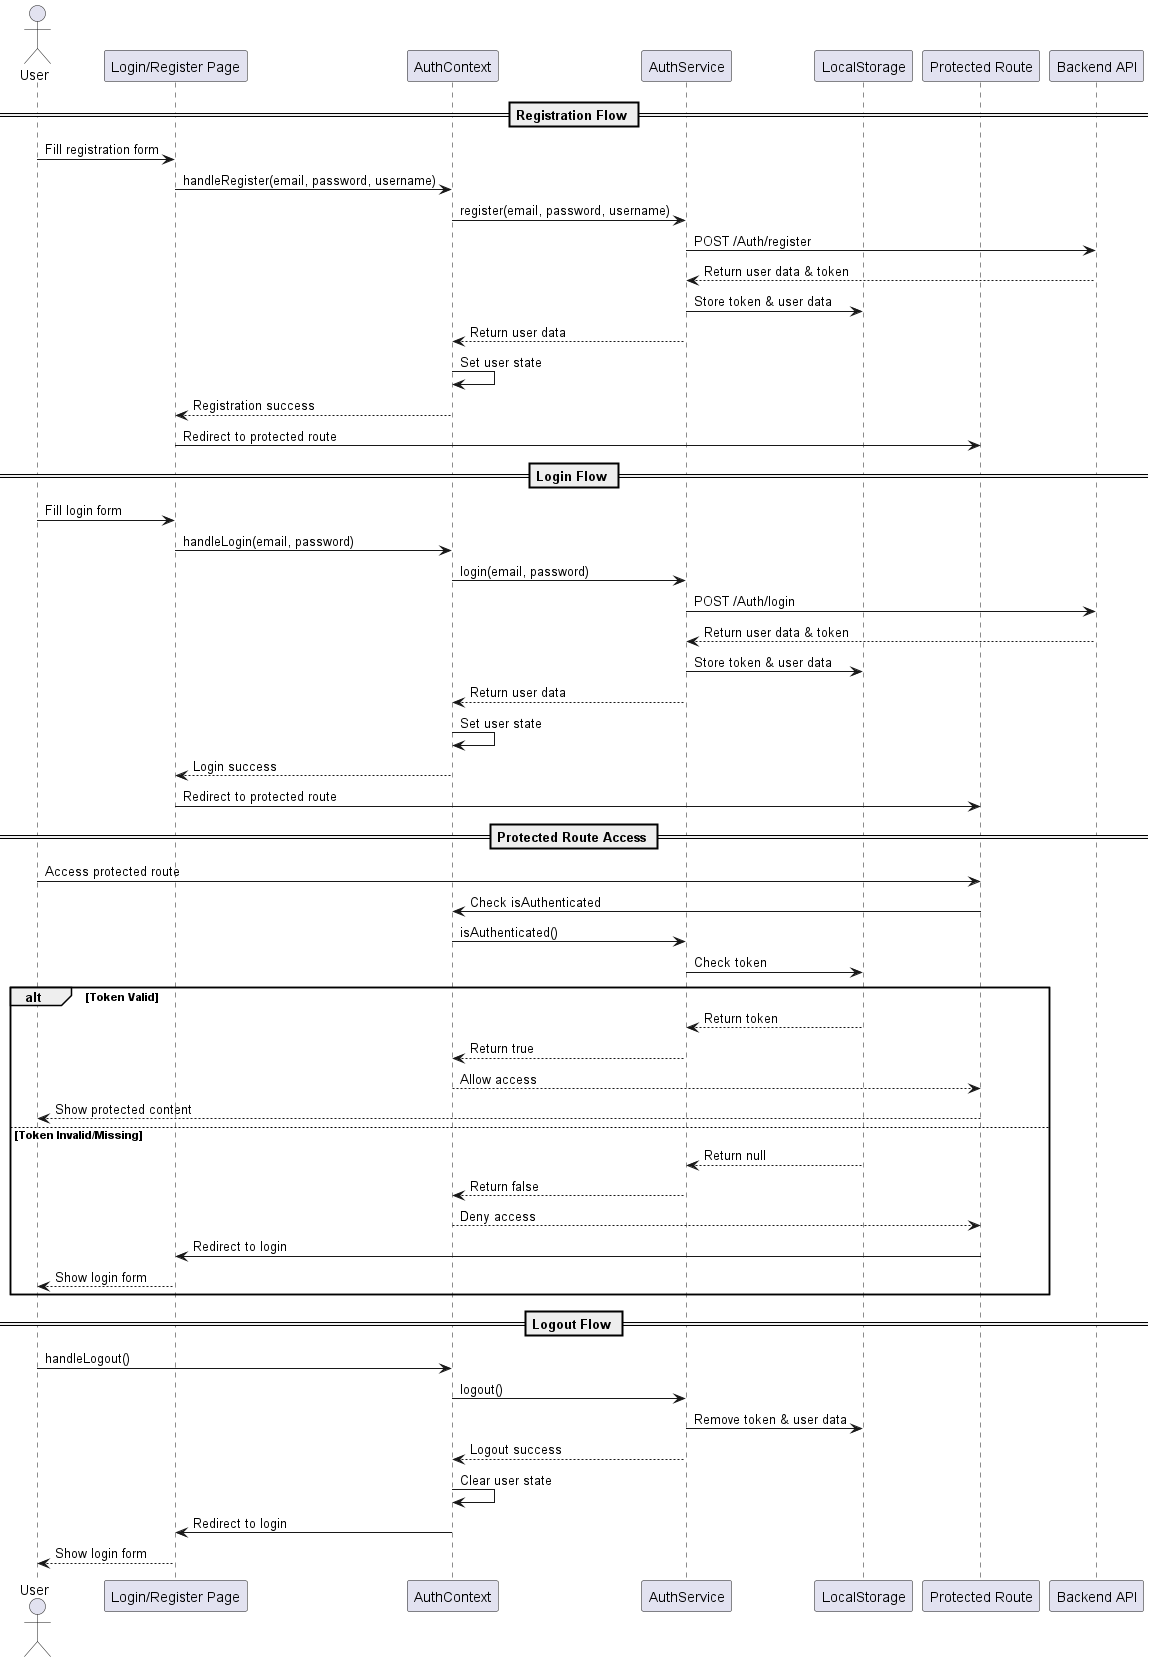
\includegraphics[width=\textwidth]{./Chapter07/figures/authentication_ui_flow.PDF}
    \caption{User Authentication Flow Through UI}
    \label{fig:authentication-ui-flow}
\end{sidewaysfigure}
\clearpage

Key authentication components include:

\begin{itemize}
  \item \textbf{LoginForm} - Handles user authentication with email/username and password
  \item \textbf{RegistrationForm} - Manages new user registration with validation
  \item \textbf{PasswordReset} - Provides password recovery functionality
  \item \textbf{ProfileEditor} - Allows users to update their profile information
  \item \textbf{UserSettings} - Provides access to account settings and preferences
\end{itemize}

These components work with the AuthContext to manage the user's authentication state and provide appropriate feedback during the authentication process.

\subsection{Model Explorer Components}

The model explorer components enable users to discover and select AI models for conversations:

\begin{sidewaysfigure}[p]
    \centering
    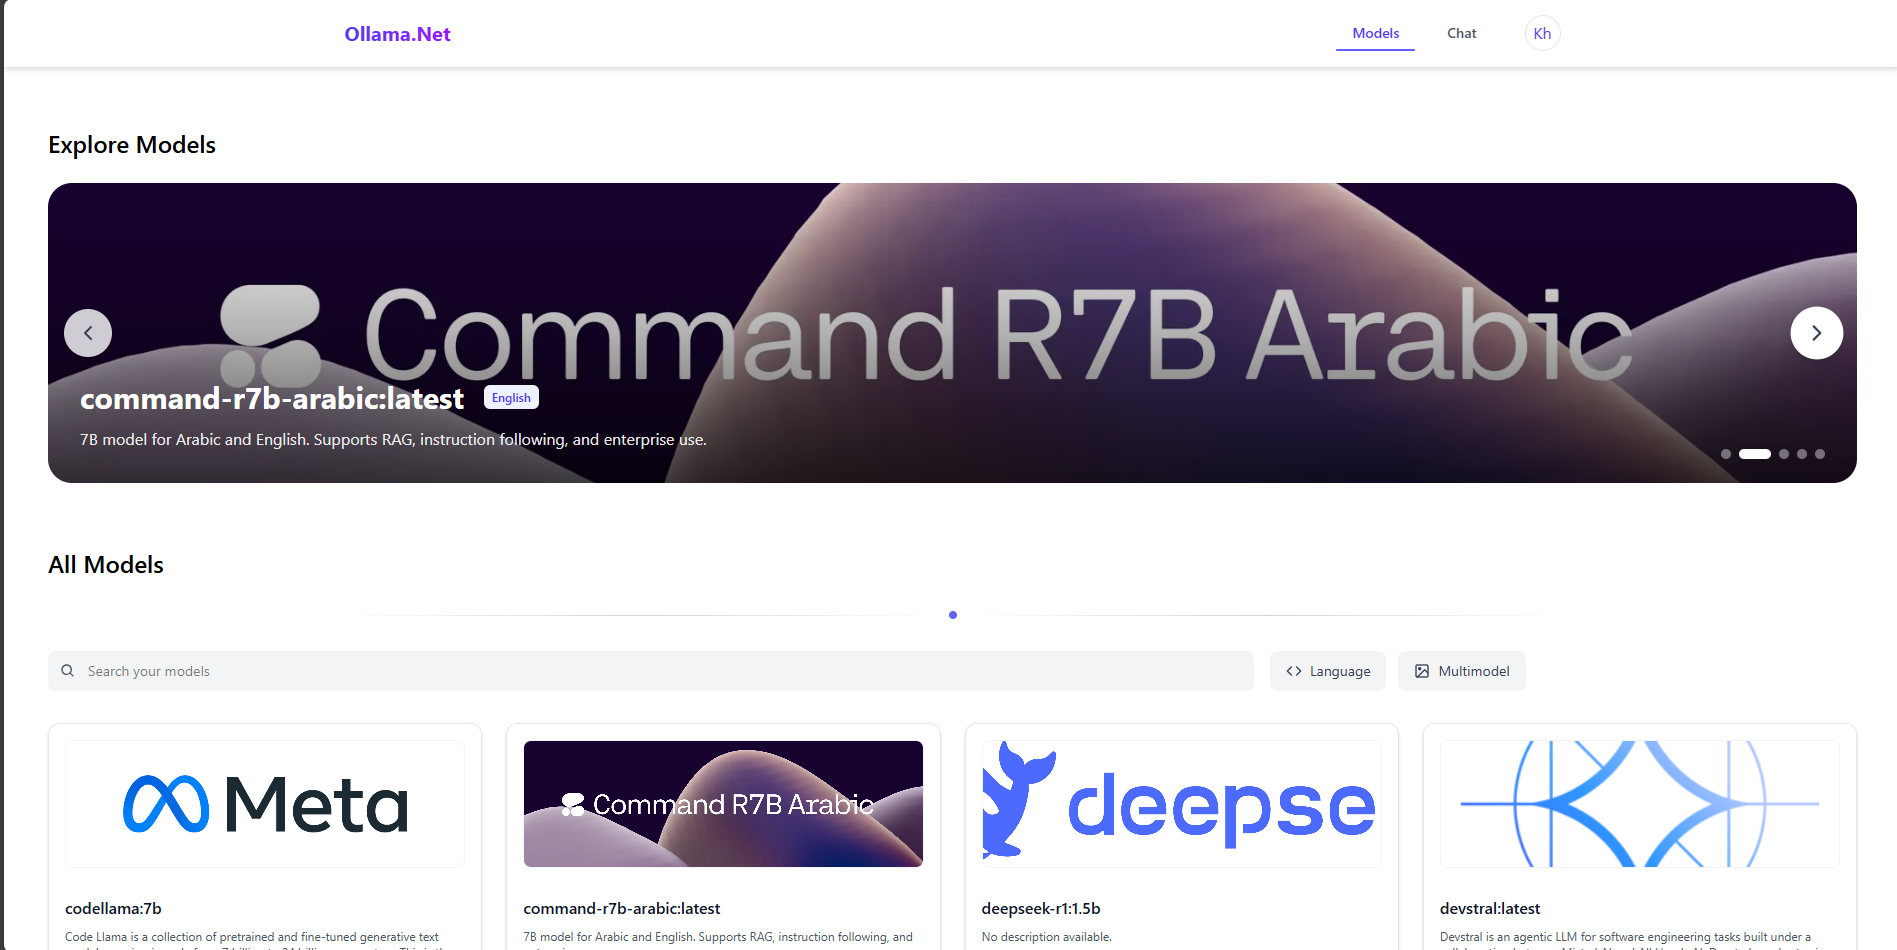
\includegraphics[width=\textwidth]{./Chapter07/figures/model_explorer_ui.PDF}
    \caption{Model Exploration Interface}
    \label{fig:model-explorer-ui}
\end{sidewaysfigure}
\clearpage

The model explorer includes these key components:

\begin{itemize}
  \item \textbf{ModelList} - Displays available models in a grid or list format
  \item \textbf{ModelCard} - Shows model information in a compact, visual format
  \item \textbf{ModelDetail} - Provides comprehensive information about a specific model
  \item \textbf{ModelFilter} - Allows filtering models by type, capability, or tags
  \item \textbf{ModelSearch} - Enables searching for models by name or description
\end{itemize}

These components help users find appropriate models for their specific needs, with visual cues indicating model capabilities and characteristics.

\subsection{Conversation Interface}

The conversation interface is the core interaction point for users to communicate with AI models:

\begin{sidewaysfigure}[p]
    \centering
      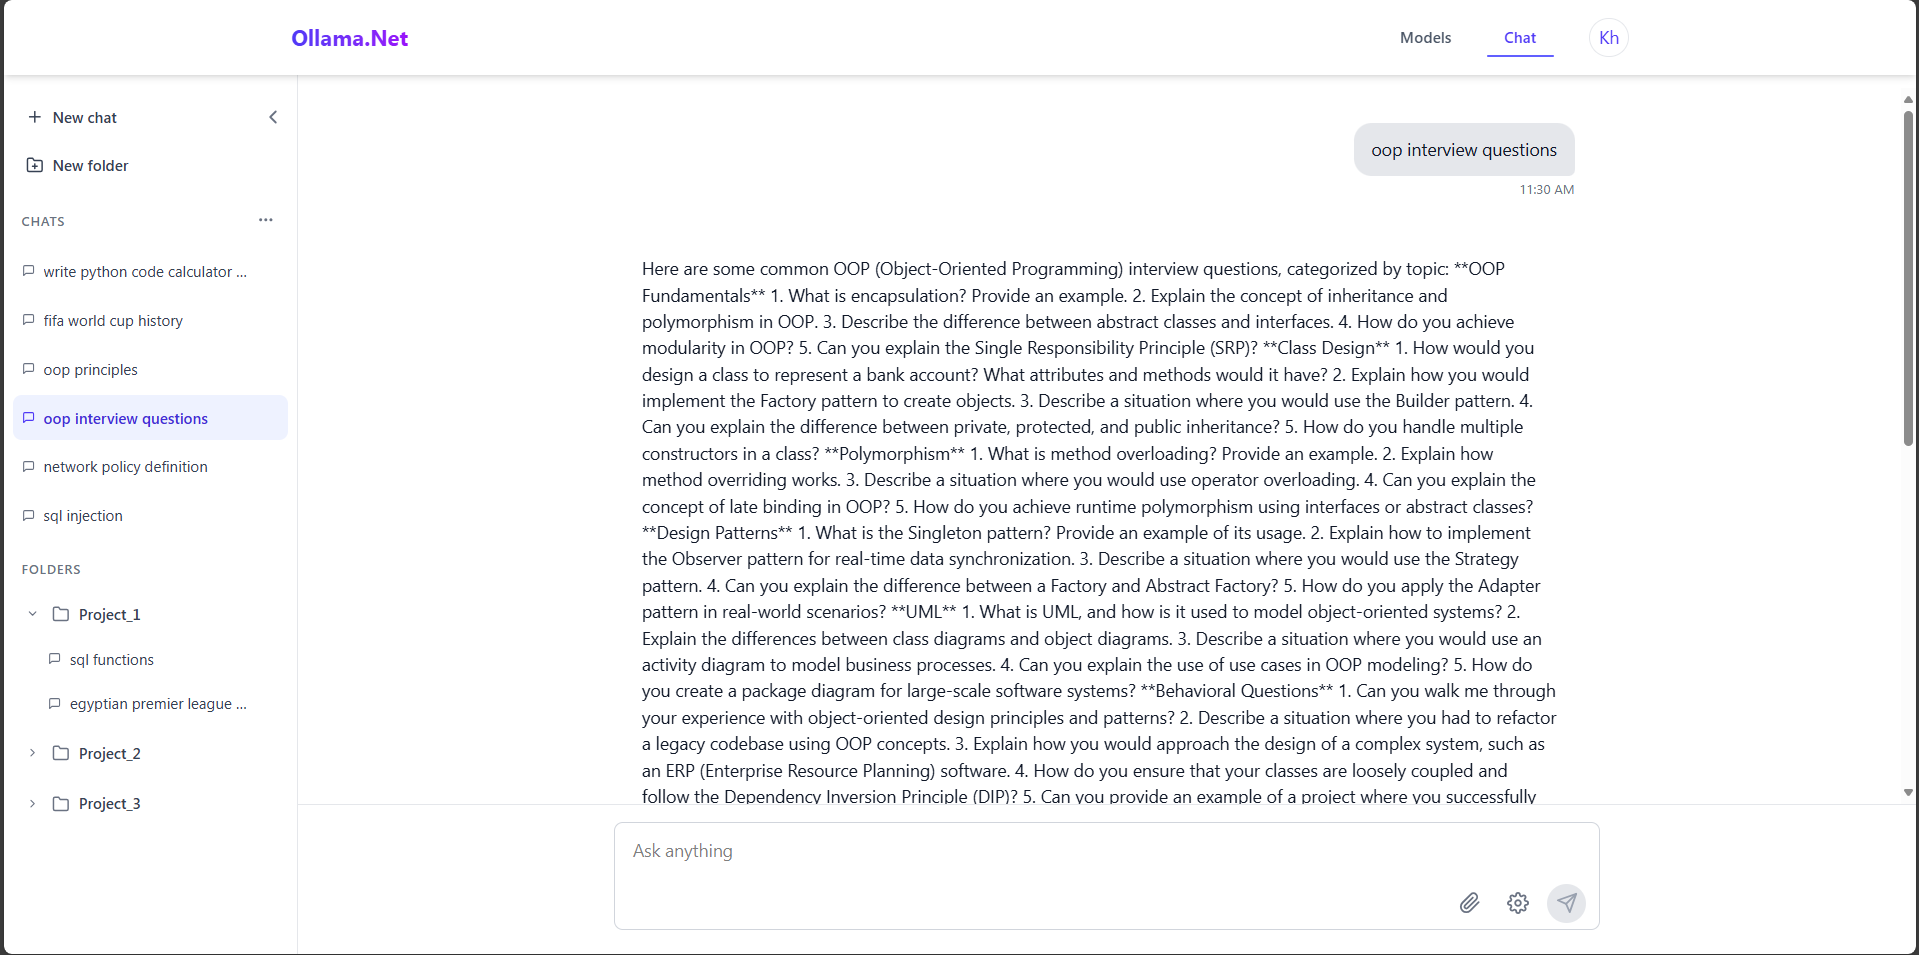
\includegraphics[width=\textwidth]{./Chapter07/figures/conversation_ui.PDF}
    \caption{Conversation Interface}
    \label{fig:conversation-ui}
\end{sidewaysfigure}
\clearpage

Key conversation components include:

\begin{itemize}
  \item \textbf{ChatContainer} - The main conversation interface container
  \item \textbf{MessageList} - Displays the history of messages in the conversation
  \item \textbf{UserMessage} - Renders user messages with appropriate styling
  \item \textbf{AIResponse} - Displays AI responses with markdown rendering
  \item \textbf{MessageInput} - Allows users to type and send messages
  \item \textbf{StreamingResponse} - Handles real-time streaming of AI responses
  \item \textbf{ConversationHeader} - Shows conversation title and actions
\end{itemize}

The conversation interface supports markdown rendering, code syntax highlighting, and streaming responses for a dynamic user experience.

\subsection{Document Management UI}

The document management interface allows users to upload and manage documents for context-enhanced conversations:

\begin{sidewaysfigure}[p]
    \centering
    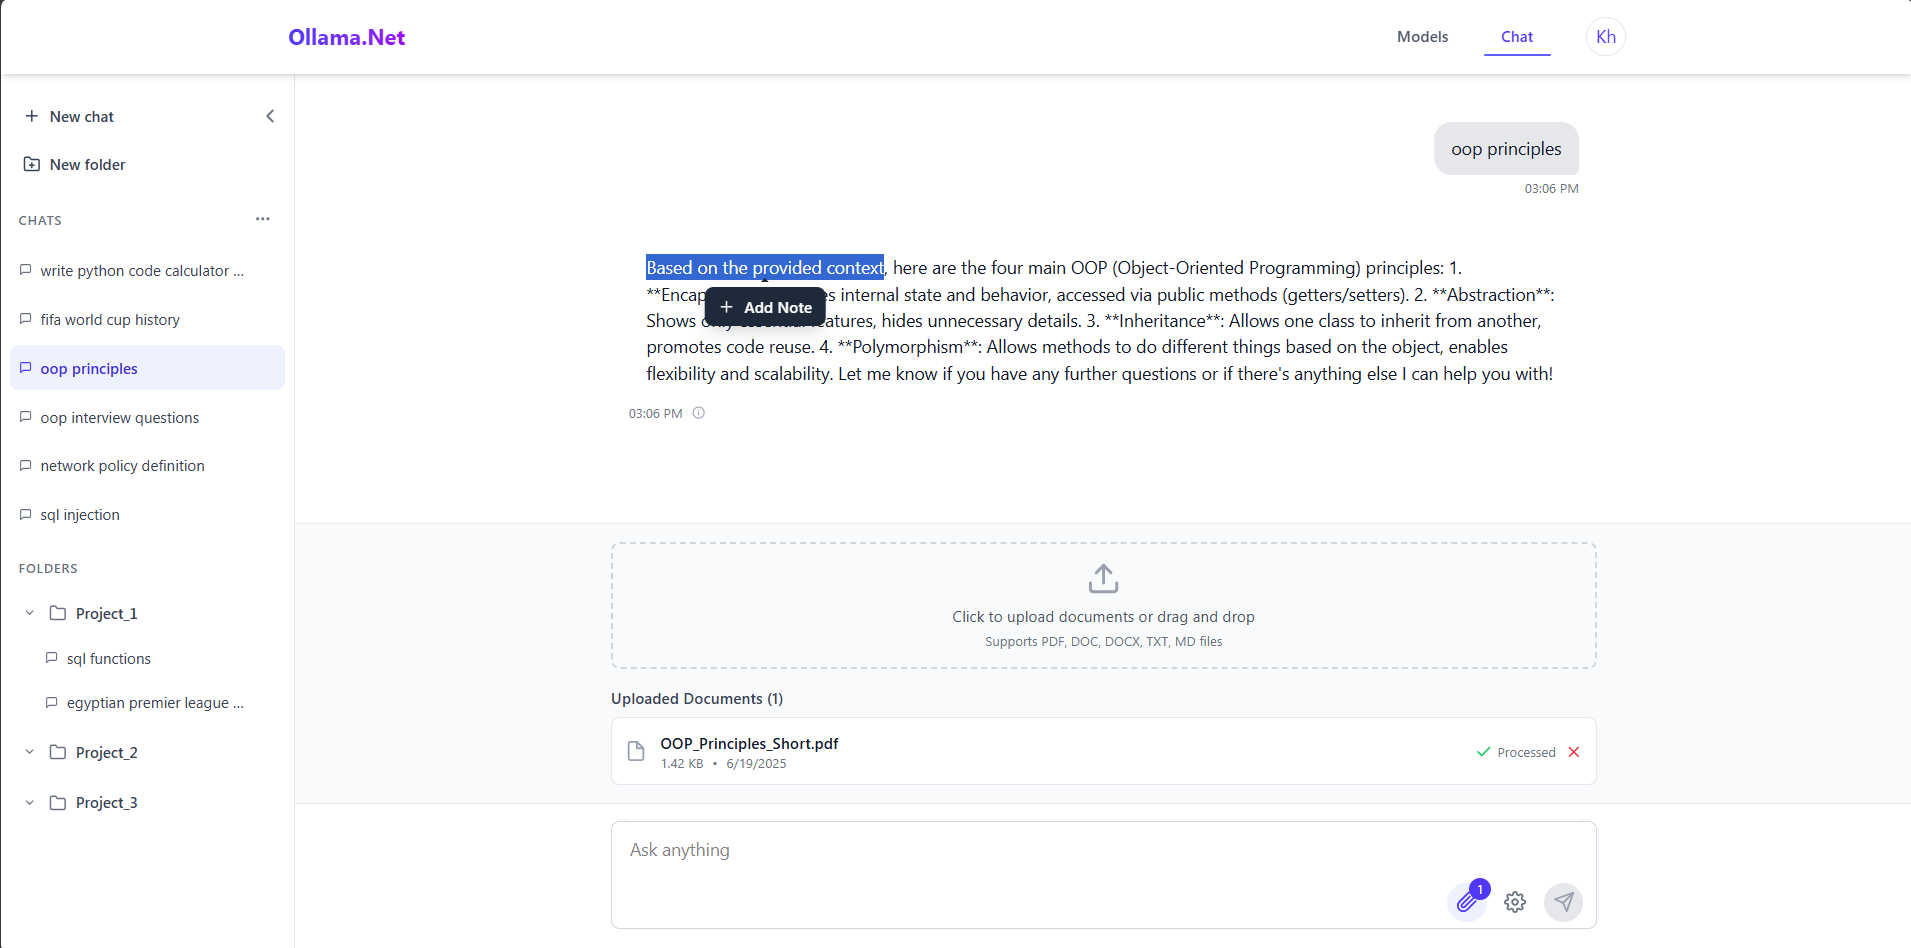
\includegraphics[width=\textwidth]{./Chapter07/figures/document_upload_ui.PDF}
    \caption{Document Upload Interface}
    \label{fig:document-upload-ui}
\end{sidewaysfigure}
\clearpage

Document management components include:

\begin{itemize}
  \item \textbf{DocumentUploader} - Handles file selection and upload
  \item \textbf{DocumentList} - Displays uploaded documents associated with a conversation
  \item \textbf{DocumentPreview} - Shows a preview of document content when possible
  \item \textbf{DocumentContext} - Indicates when a document is being used for context
\end{itemize}

These components integrate with the conversation interface to enhance AI responses with document context.

\subsection{Folder Organization System}

The folder organization system helps users manage their conversations in a structured way:

\begin{sidewaysfigure}[p]
    \centering
    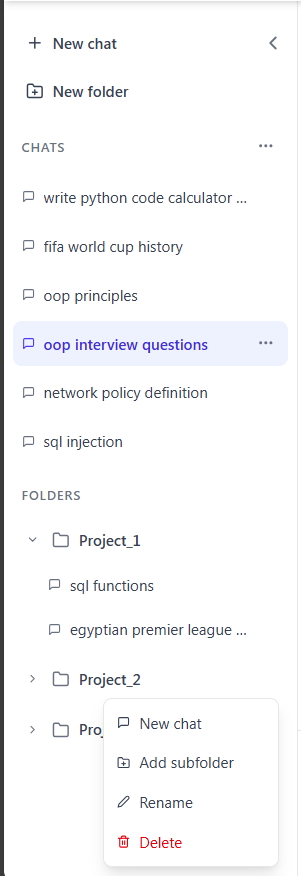
\includegraphics[width=\textwidth,height=0.8\textheight,keepaspectratio]{./Chapter07/figures/folder_organization_ui.PDF}
    \caption{Folder Organization System}
    \label{fig:folder-organization-ui}
\end{sidewaysfigure}
\clearpage

Key folder organization components include:

\begin{itemize}
  \item \textbf{FolderTree} - Displays folders in a hierarchical structure
  \item \textbf{FolderItem} - Represents a single folder with actions
  \item \textbf{ConversationItem} - Shows a conversation within a folder
  \item \textbf{FolderActions} - Provides options to create, rename, and delete folders
  \item \textbf{DragDropContext} - Enables drag-and-drop organization of conversations
\end{itemize}

The folder system allows users to categorize and easily retrieve past conversations, improving the organization of their AI interactions.

\section{State Management}

State management in the Ollama UI application is implemented using a combination of React's Context API, custom hooks, and React Query. This approach provides a balance between simplicity and powerful state management capabilities.

\begin{sidewaysfigure}[p]
    \centering
    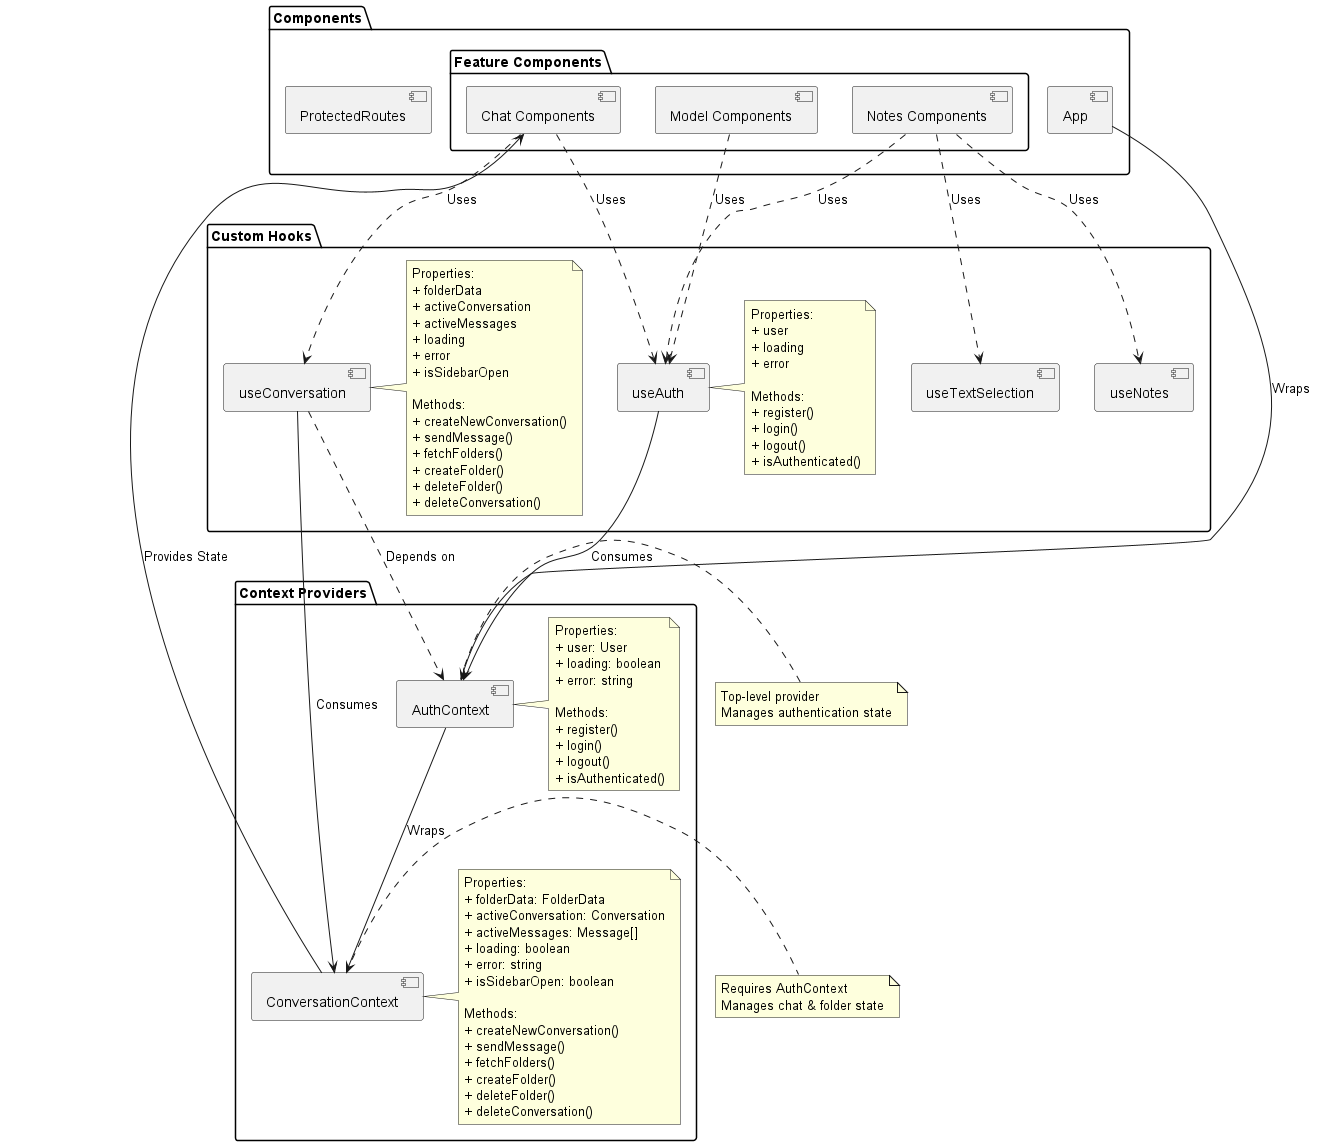
\includegraphics[width=\textwidth]{./Chapter07/figures/context_provider_hierarchy.PDF}
    \caption{Context Provider Hierarchy}
    \label{fig:context-provider-hierarchy}
\end{sidewaysfigure}
\clearpage

\subsection{React Context Implementation}

The application uses several context providers to manage global state:

\begin{itemize}
  \item \textbf{AuthContext} - Manages user authentication state
  \item \textbf{ConversationContext} - Handles conversation data and interactions
  \item \textbf{ModelContext} - Provides access to available AI models
  \item \textbf{UIContext} - Manages UI state like theme preferences and sidebar visibility
  \item \textbf{NotificationContext} - Controls application notifications and alerts
\end{itemize}

These context providers are organized hierarchically, with the AuthContext at the highest level since many other contexts depend on the authentication state.

Context providers implement proper memoization to prevent unnecessary re-renders:

\begin{verbatim}
// Example of a context provider with memoization
export const ConversationProvider = ({ children }) => {
  const [conversations, setConversations] = useState([]);
  const [activeConversation, setActiveConversation] = useState(null);
  
  // Memoized value to prevent unnecessary re-renders
  const value = useMemo(() => ({
    conversations,
    activeConversation,
    setActiveConversation,
    // Other functions...
  }), [conversations, activeConversation]);
  
  return (
    <ConversationContext.Provider value={value}>
      {children}
    </ConversationContext.Provider>
  );
};
\end{verbatim}

\subsection{Custom Hooks}

The application encapsulates complex logic and state management in custom hooks, which provide a clean API for components to interact with:

\begin{itemize}
  \item \textbf{useAuth} - Provides authentication functions and user state
  \item \textbf{useConversation} - Manages conversation data and operations
  \item \textbf{useModels} - Handles model discovery and selection
  \item \textbf{useDocuments} - Manages document upload and retrieval
  \item \textbf{useNotifications} - Controls displaying notifications to users
\end{itemize}

These hooks abstract away the implementation details of state management, making components cleaner and more focused on their UI responsibilities:

\begin{verbatim}
// Example of a custom hook that uses context
export const useConversation = () => {
  const context = useContext(ConversationContext);
  
  if (!context) {
    throw new Error('useConversation must be used within a ConversationProvider');
  }
  
  // Additional derived state or functions can be added here
  const startNewConversation = useCallback(async (modelId) => {
    // Implementation details...
  }, [context.createConversation]);
  
  return {
    ...context,
    startNewConversation,
  };
};
\end{verbatim}

\subsection{API Integration}

The application integrates with backend APIs using React Query, which provides data fetching, caching, and synchronization:

\begin{sidewaysfigure}[p]
    \centering
    \includegraphics[width=\textwidth]{./Chapter07/figures/api_integration_pattern.PDF}
    \caption{Frontend-API Integration Pattern}
    \label{fig:api-integration-pattern}
\end{sidewaysfigure}
\clearpage

API integration is implemented through service modules that encapsulate API communication:

\begin{itemize}
  \item \textbf{authService} - Handles authentication API requests
  \item \textbf{conversationService} - Manages conversation-related API calls
  \item \textbf{modelService} - Handles model-related API requests
  \item \textbf{documentService} - Manages document upload and retrieval
\end{itemize}

These services use Axios for HTTP requests and implement consistent error handling:

\begin{verbatim}
// Example of an API service
const conversationService = {
  getConversations: async () => {
    try {
      const response = await axios.get('/api/conversations');
      return response.data;
    } catch (error) {
      handleApiError(error);
      throw error;
    }
  },
  
  // Other API methods...
};
\end{verbatim}

\subsection{Caching Strategies}

The application implements several caching strategies to optimize performance:

\begin{itemize}
  \item \textbf{React Query Caching} - Automatically caches API responses with configurable expiration
  \item \textbf{Local Storage Persistence} - Certain data is persisted to local storage for offline access
  \item \textbf{Memory Caching} - In-memory caching for frequently accessed data
  \item \textbf{Optimistic Updates} - UI updates immediately while changes are being saved
\end{itemize}

Caching is particularly important for model information and conversation history, which are accessed frequently during user sessions.

\section{UI/UX Design Patterns}

The Ollama UI application follows modern UI/UX design patterns to provide an intuitive, responsive, and accessible user experience. These patterns ensure consistency across the application and align with user expectations for web applications.

\begin{sidewaysfigure}[p]
    \centering
    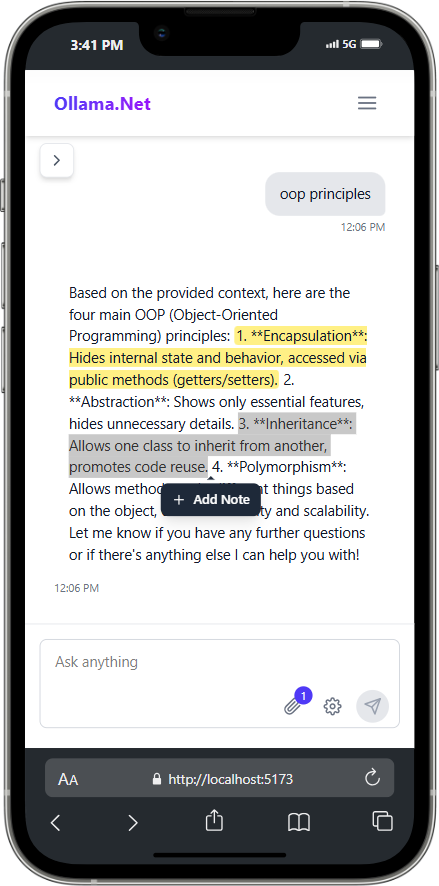
\includegraphics[width=\textwidth,height=0.8\textheight,keepaspectratio]{./Chapter07/figures/mobile_responsive_views.PDF}
    \caption{Mobile Responsive Views}
    \label{fig:mobile-responsive-views}
\end{sidewaysfigure}
\clearpage

\subsection{Responsive Design Implementation}

The application implements responsive design using Tailwind CSS's utility classes and responsive modifiers:

\begin{itemize}
  \item \textbf{Mobile-First Approach} - Design starts with mobile layouts and expands for larger screens
  \item \textbf{Responsive Breakpoints} - Consistent breakpoints for small, medium, and large screens
  \item \textbf{Fluid Typography} - Text sizes adjust based on screen size
  \item \textbf{Adaptive Layouts} - Components reorganize based on available space
  \item \textbf{Touch-Friendly Targets} - Interactive elements sized appropriately for touch devices
\end{itemize}

The responsive implementation ensures that users have a consistent experience across devices, from mobile phones to desktop computers.

\subsection{Accessibility Considerations}

The application incorporates accessibility best practices to ensure usability for all users:

\begin{itemize}
  \item \textbf{Semantic HTML} - Using appropriate HTML elements for their intended purpose
  \item \textbf{ARIA Attributes} - Adding ARIA roles and attributes where necessary
  \item \textbf{Keyboard Navigation} - Ensuring all interactive elements are keyboard accessible
  \item \textbf{Color Contrast} - Maintaining sufficient contrast ratios for text and interactive elements
  \item \textbf{Focus Management} - Properly managing focus, especially in modal dialogs
  \item \textbf{Screen Reader Support} - Adding alternative text for images and descriptive labels
\end{itemize}

These practices ensure that the application is usable by people with various disabilities, including visual, motor, and cognitive impairments.

\subsection{Loading States and Transitions}

The application provides visual feedback during asynchronous operations:

\begin{itemize}
  \item \textbf{Loading Spinners} - Indicate that data is being fetched
  \item \textbf{Skeleton Screens} - Show placeholder content while data loads
  \item \textbf{Progress Indicators} - Display progress for operations like file uploads
  \item \textbf{Transition Animations} - Smooth transitions between UI states
  \item \textbf{Button Loading States} - Visual feedback when buttons trigger async operations
\end{itemize}

These loading states and transitions provide a sense of continuity and prevent user confusion during operations that take time to complete.

\subsection{Error Handling Patterns}

The application implements consistent error handling patterns:

\begin{itemize}
  \item \textbf{Inline Validation} - Form fields validate input and show errors inline
  \item \textbf{Toast Notifications} - Temporary notifications for non-critical errors
  \item \textbf{Error Boundaries} - Catch and display component errors gracefully
  \item \textbf{Fallback UI} - Show alternative content when primary content fails to load
  \item \textbf{Retry Mechanisms} - Allow users to retry failed operations
  \item \textbf{Clear Error Messages} - Provide understandable error messages with possible solutions
\end{itemize}

These error handling patterns ensure that users understand what went wrong and how to recover, maintaining a positive user experience even when errors occur.

\section{Frontend Performance Optimization}

The Ollama UI application implements various performance optimization techniques to ensure a responsive and efficient user experience, even when dealing with complex interactions and large datasets.

\begin{sidewaysfigure}[p]
    \centering
    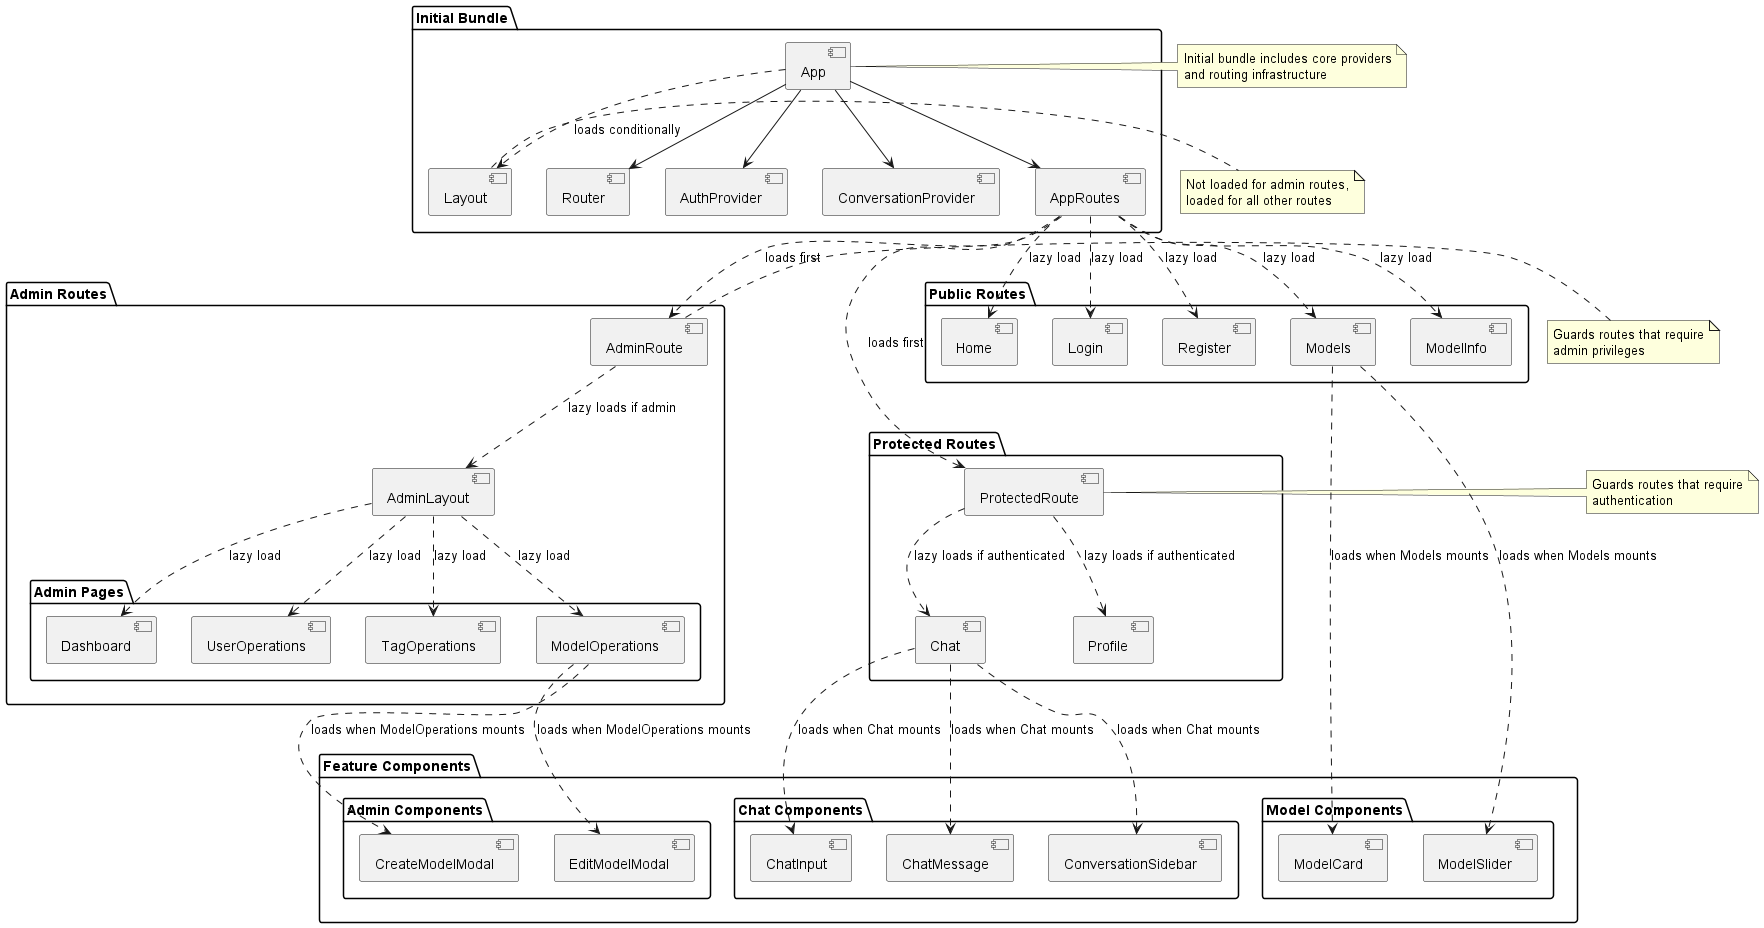
\includegraphics[width=\textwidth]{./Chapter07/figures/component_lazy_loading.PDF}
    \caption{Component Lazy Loading Pattern}
    \label{fig:component-lazy-loading}
\end{sidewaysfigure}
\clearpage

\subsection{Component Lazy Loading}

The application uses code splitting and lazy loading to reduce the initial bundle size and improve load times:

\begin{itemize}
  \item \textbf{Route-Based Code Splitting} - Each route loads its components on demand
  \item \textbf{Dynamic Imports} - Components are imported dynamically when needed
  \item \textbf{Suspense Integration} - React Suspense provides fallback UI during loading
  \item \textbf{Prefetching} - Critical components are prefetched when likely to be needed
\end{itemize}

This approach significantly reduces the initial load time of the application while ensuring a smooth user experience:

\begin{verbatim}
// Example of lazy loading a component
const ModelExplorer = React.lazy(() => import('./ModelExplorer'));

// Usage with Suspense
<Suspense fallback={<LoadingSpinner />}>
  <ModelExplorer />
</Suspense>
\end{verbatim}

\subsection{Resource Optimization}

The application optimizes resource loading and usage:

\begin{itemize}
  \item \textbf{Image Optimization} - Images are compressed and served in appropriate formats
  \item \textbf{Asset Bundling} - Vite optimizes asset bundling for production
  \item \textbf{Code Minification} - JavaScript and CSS are minified for production
  \item \textbf{Tree Shaking} - Unused code is eliminated from the production bundle
  \item \textbf{Font Loading} - Fonts are loaded efficiently with proper fallbacks
\end{itemize}

These optimizations reduce the overall resource footprint and improve loading performance, particularly on slower networks.

\subsection{Rendering Performance}

The application implements several techniques to optimize rendering performance:

\begin{itemize}
  \item \textbf{Memoization} - React.memo and useMemo prevent unnecessary re-renders
  \item \textbf{Virtualization} - Virtual lists for displaying large datasets efficiently
  \item \textbf{Throttling and Debouncing} - Control frequency of expensive operations
  \item \textbf{Web Workers} - Offload heavy computations to background threads
  \item \textbf{Optimized Event Handlers} - Event handlers are debounced or throttled when appropriate
\end{itemize}

These techniques ensure smooth UI interactions, even when dealing with complex components or large data sets:

\begin{verbatim}
// Example of memoization to optimize rendering
const MemoizedConversationItem = React.memo(
  ConversationItem, 
  (prevProps, nextProps) => {
    return prevProps.id === nextProps.id && 
           prevProps.lastUpdated === nextProps.lastUpdated;
  }
);
\end{verbatim}

\subsection{Cache Management}

The application implements strategic cache management to balance performance and data freshness:

\begin{itemize}
  \item \textbf{React Query Caching} - Configurable caching of API responses
  \item \textbf{Stale-While-Revalidate} - Show cached data while fetching fresh data
  \item \textbf{Cache Invalidation} - Strategically invalidate caches when data changes
  \item \textbf{Persistence} - Certain caches persist across sessions
  \item \textbf{Cache Prioritization} - Frequently accessed data is prioritized in cache
\end{itemize}

Effective cache management significantly improves perceived performance by reducing loading times for frequently accessed data, while ensuring that users see up-to-date information.

\begin{mdframed}[
  linewidth=0.5pt,
  frametitle={Terminology},
  frametitlefont=\normalfont\bfseries,
  backgroundcolor=gray!10,
  roundcorner=4pt,
  skipabove=7pt,
  skipbelow=7pt
]
\begin{description}
  \item[React Context:] A method to pass data through the component tree without having to pass props down manually at every level.
  \item[Lazy Loading:] A design pattern where resources are loaded only when needed, improving initial load performance.
  \item[Memoization:] An optimization technique that stores the results of expensive function calls and returns the cached result when the same inputs occur again.
  \item[React Query:] A library for fetching, caching, and updating asynchronous data in React applications.
  \item[Tailwind CSS:] A utility-first CSS framework for rapidly building custom user interfaces.
\end{description}
\end{mdframed}

\begin{sidewaysfigure}[p]
    \centering
    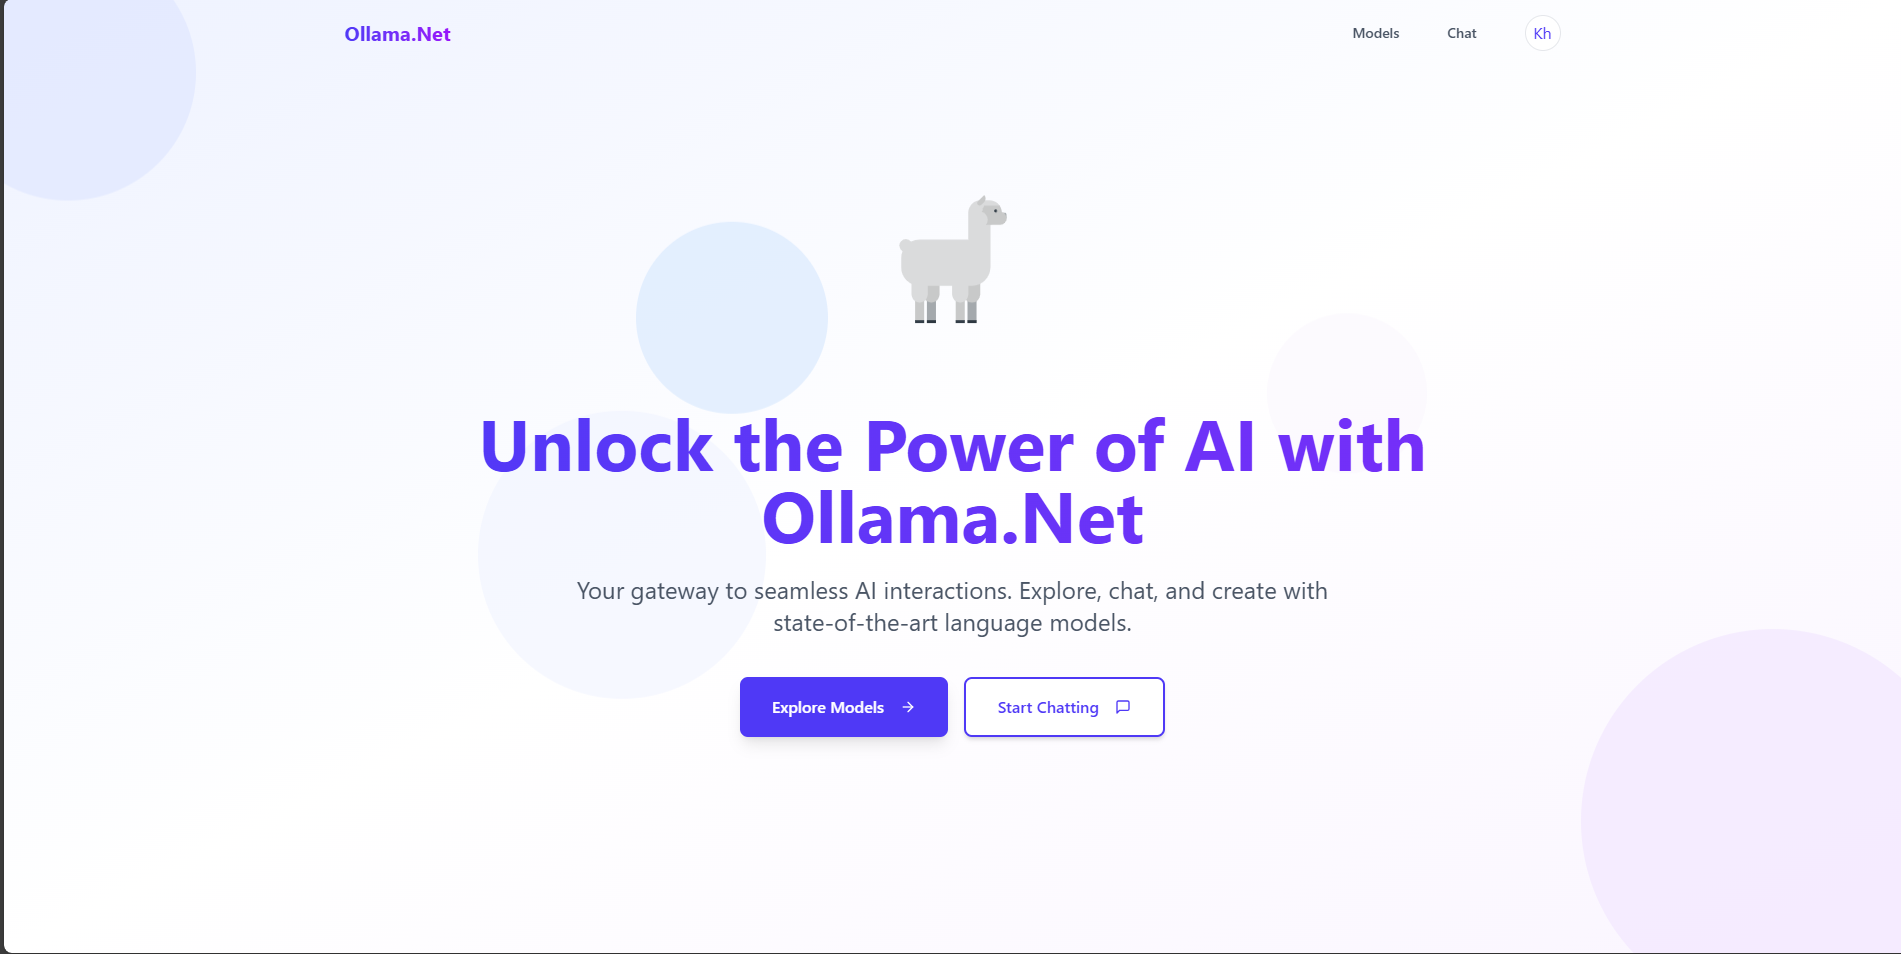
\includegraphics[width=\textwidth]{./Chapter07/figures/3.PDF}
    \caption{UI Figure 3}
    \label{fig:ui-figure-3}
\end{sidewaysfigure}
\clearpage

\begin{sidewaysfigure}[p]
    \centering
    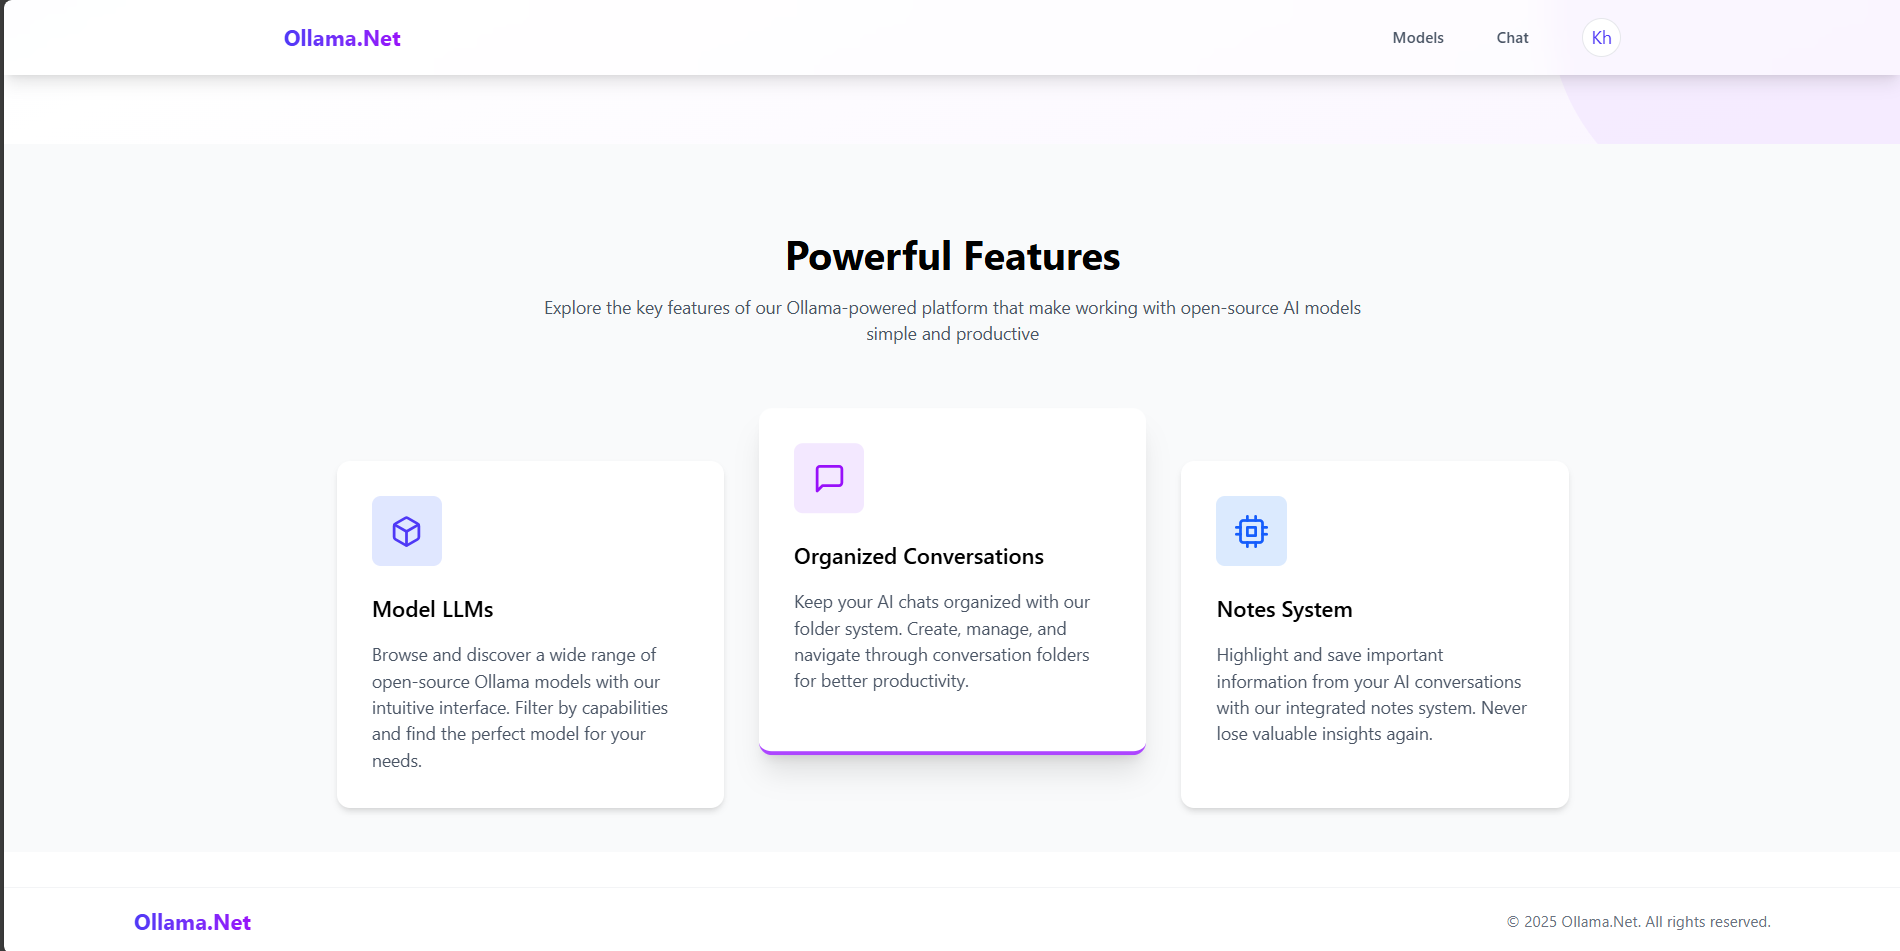
\includegraphics[width=\textwidth]{./Chapter07/figures/4.PDF}
    \caption{UI Figure 4}
    \label{fig:ui-figure-4}
\end{sidewaysfigure}
\clearpage

\begin{sidewaysfigure}[p]
    \centering
    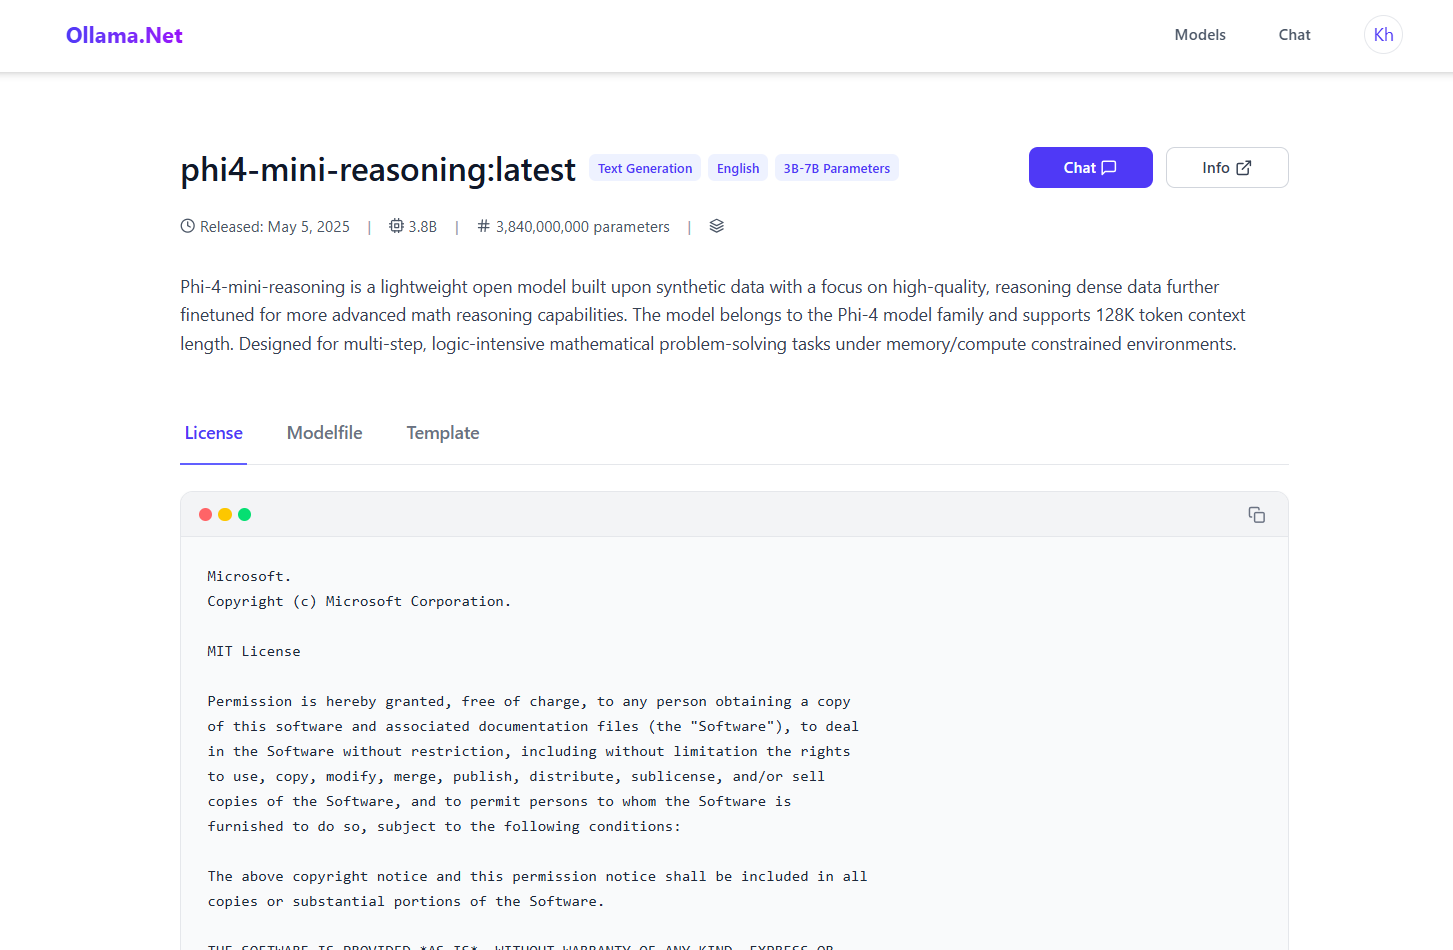
\includegraphics[width=\textwidth]{./Chapter07/figures/9.PDF}
    \caption{UI Figure 9}
    \label{fig:ui-figure-9}
\end{sidewaysfigure}
\clearpage

\begin{sidewaysfigure}[p]
    \centering
    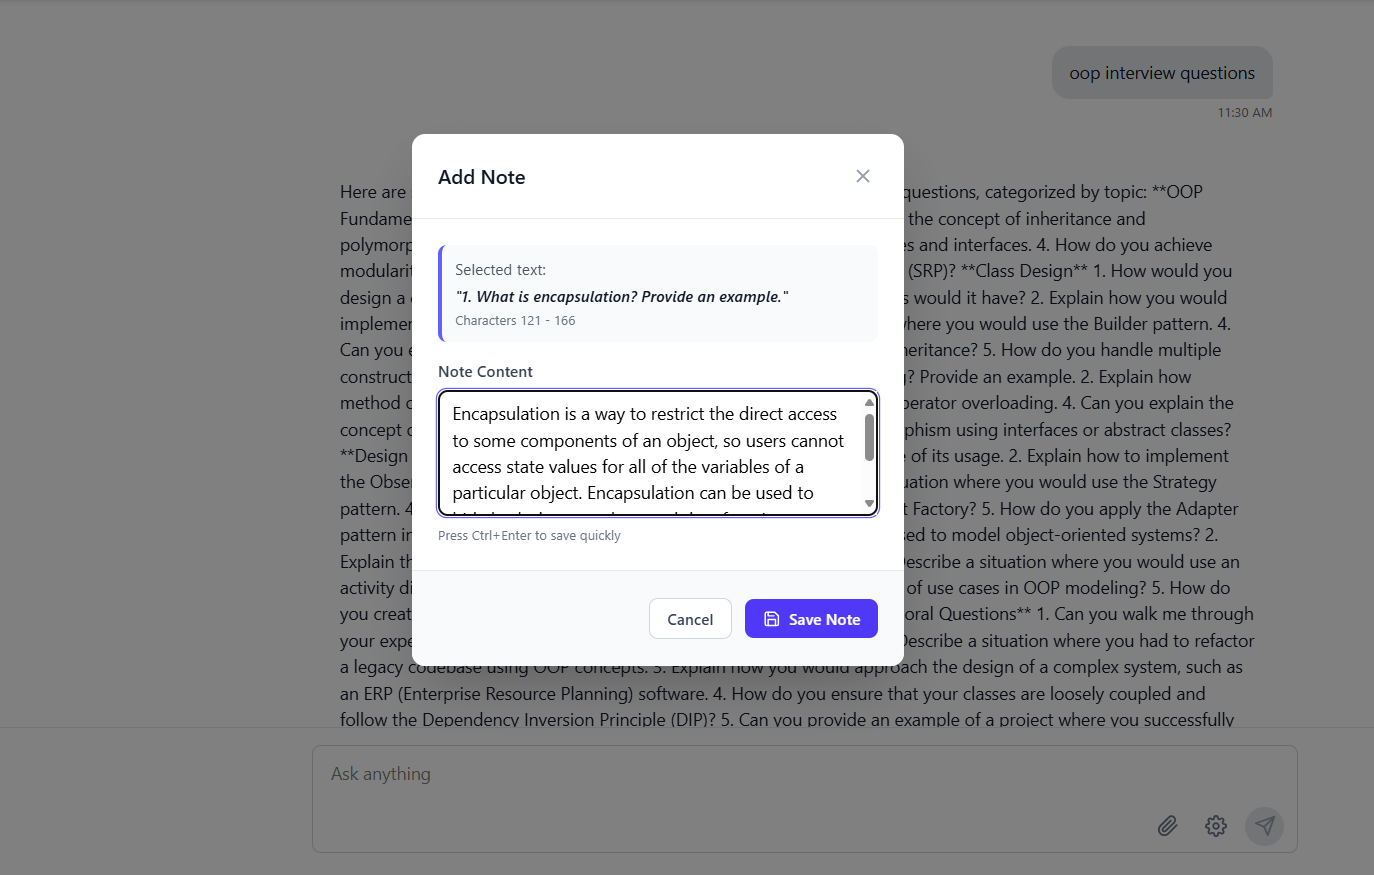
\includegraphics[width=\textwidth]{./Chapter07/figures/14.PDF}
    \caption{UI Figure 14}
    \label{fig:ui-figure-14}
\end{sidewaysfigure}
\clearpage

\begin{sidewaysfigure}[p]
    \centering
    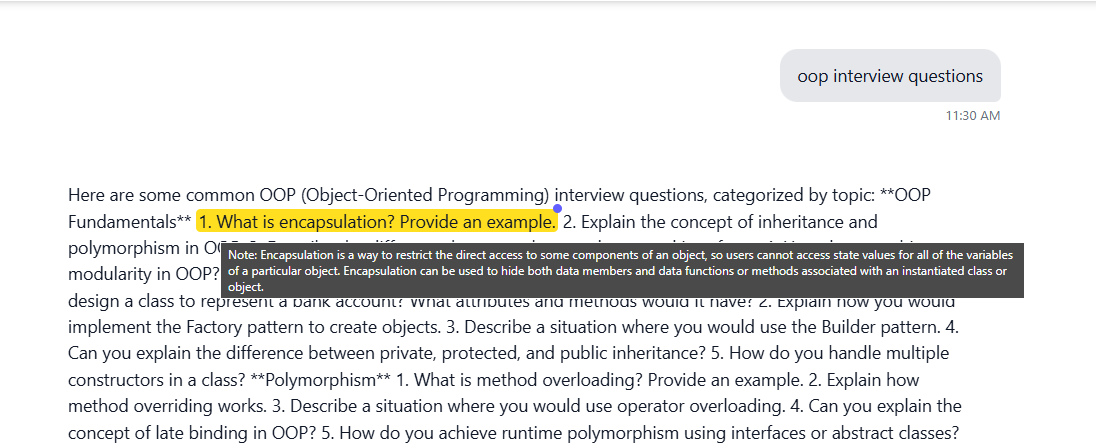
\includegraphics[width=\textwidth]{./Chapter07/figures/15.PDF}
    \caption{UI Figure 15}
    \label{fig:ui-figure-15}
\end{sidewaysfigure}
\clearpage

\begin{sidewaysfigure}[p]
    \centering
    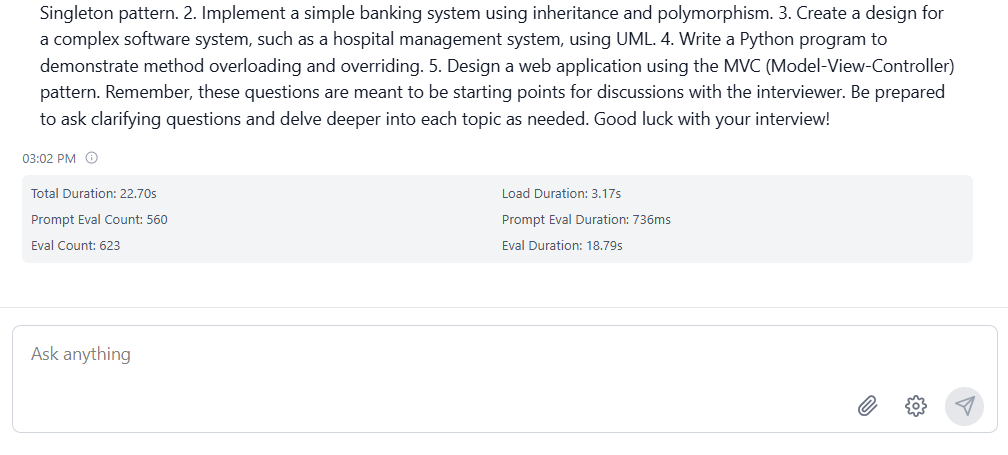
\includegraphics[width=\textwidth]{./Chapter07/figures/17.PDF}
    \caption{UI Figure 17}
    \label{fig:ui-figure-17}
\end{sidewaysfigure}
\clearpage

\begin{sidewaysfigure}[p]
    \centering
    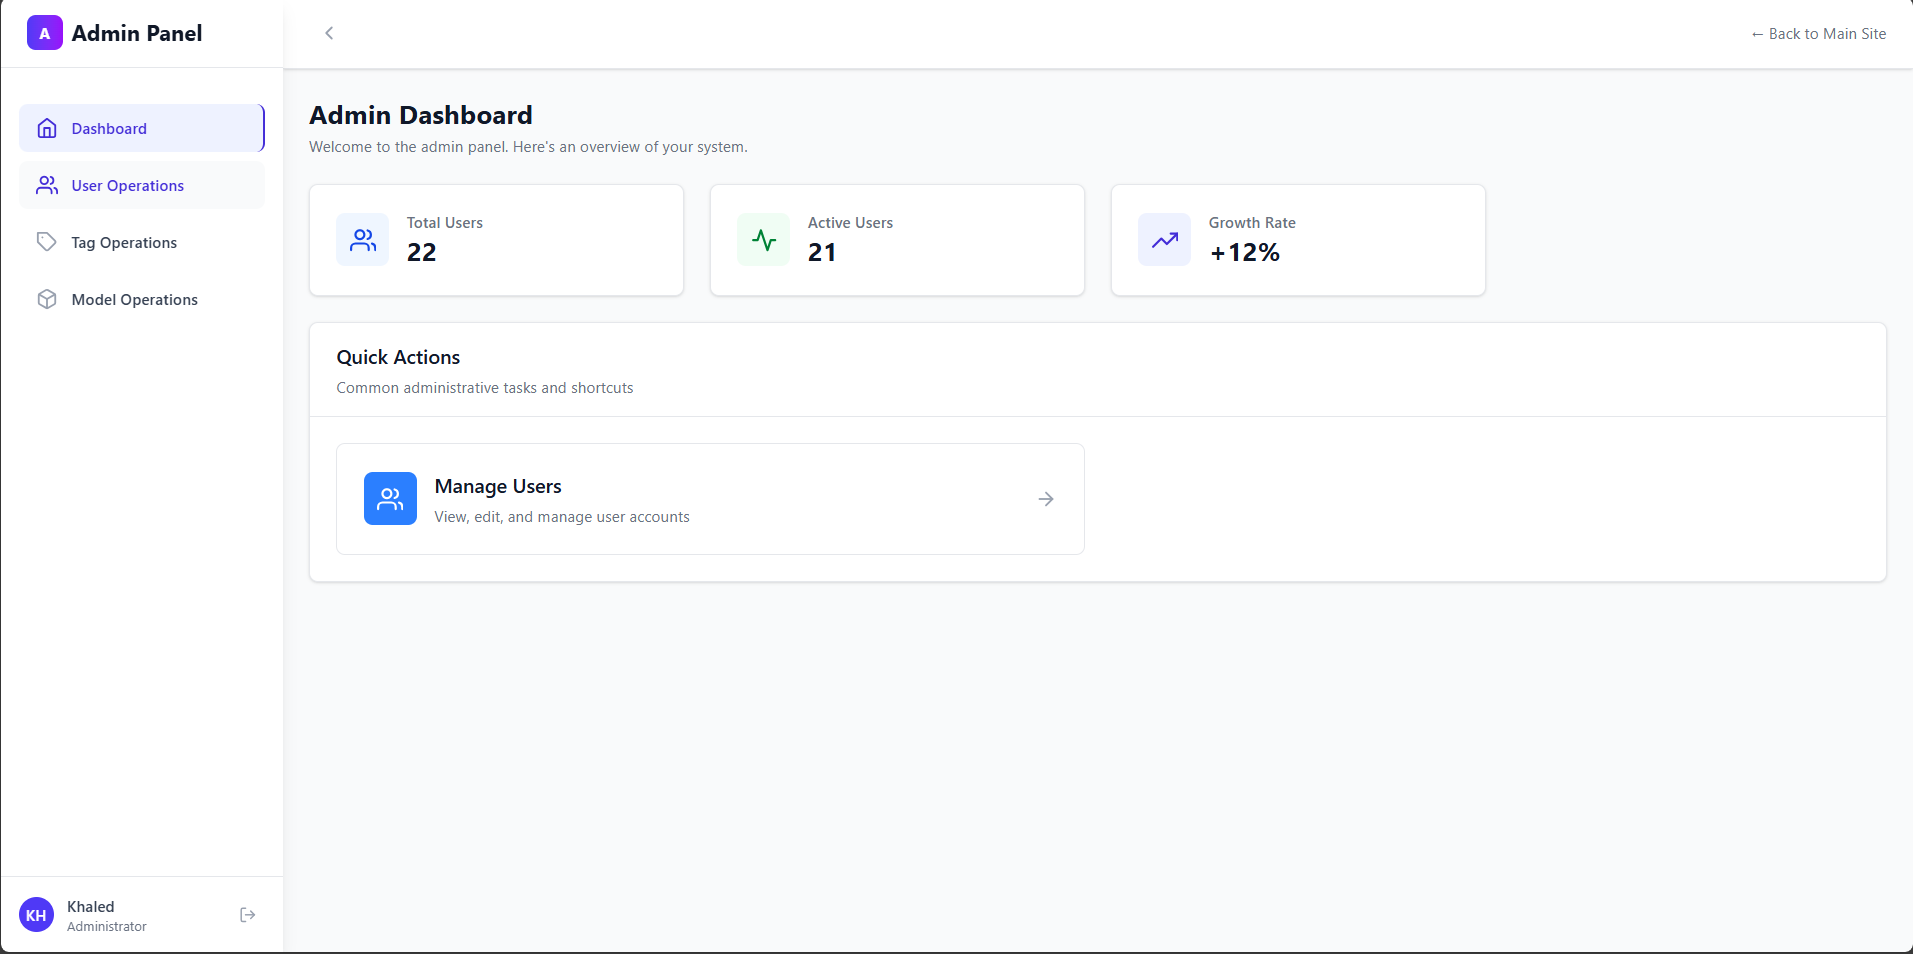
\includegraphics[width=\textwidth]{./Chapter07/figures/20.PDF}
    \caption{UI Figure 20}
    \label{fig:ui-figure-20}
\end{sidewaysfigure}
\clearpage

\begin{sidewaysfigure}[p]
    \centering
    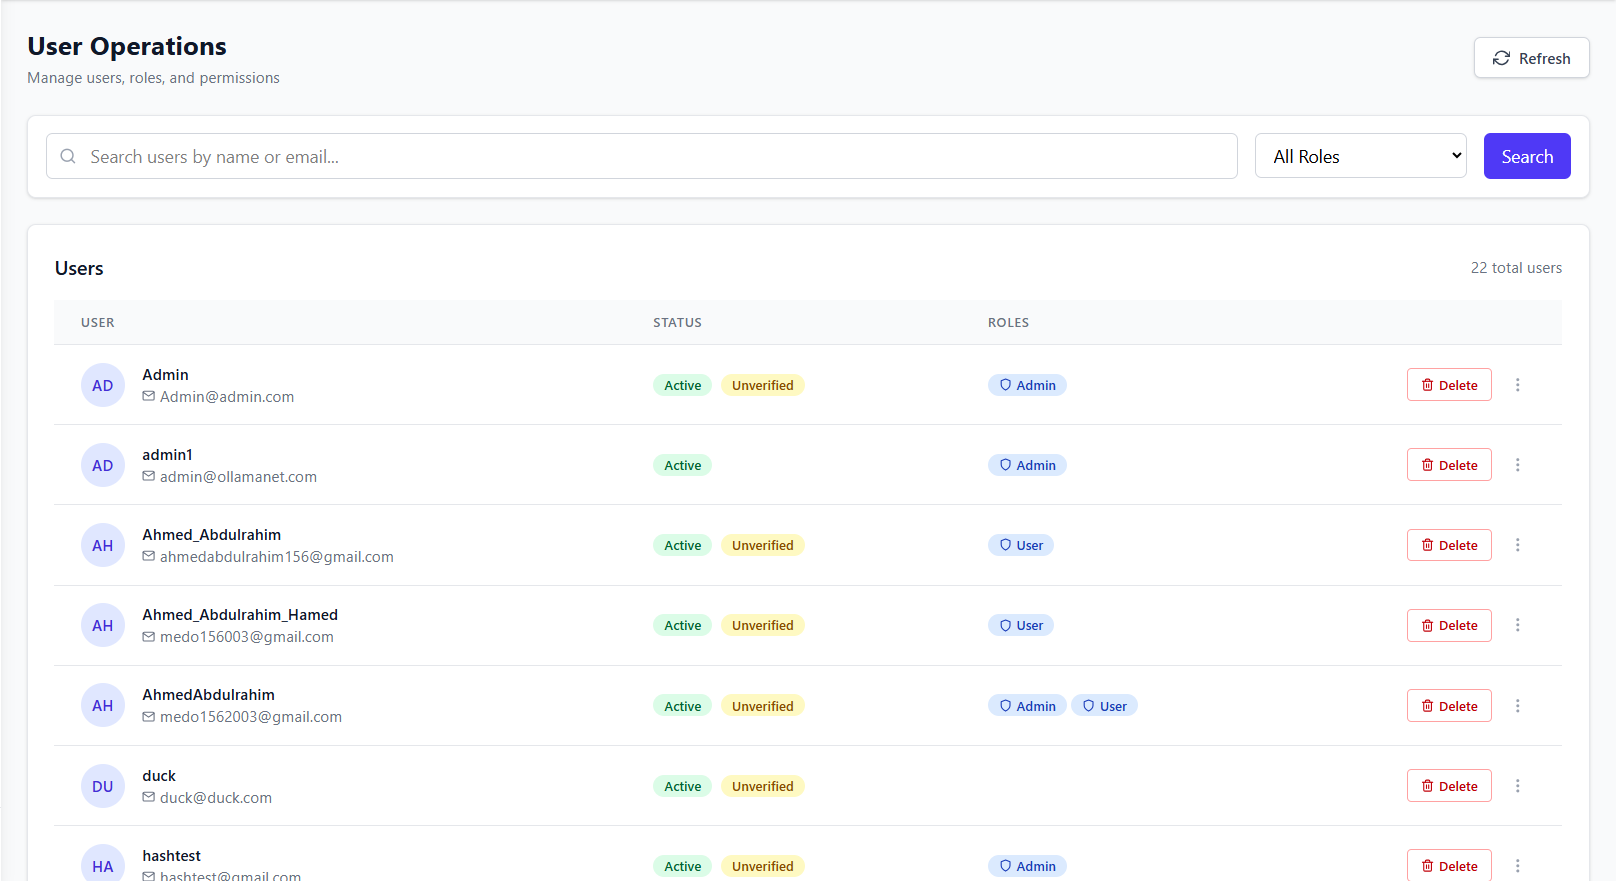
\includegraphics[width=\textwidth]{./Chapter07/figures/21.PDF}
    \caption{UI Figure 21}
    \label{fig:ui-figure-21}
\end{sidewaysfigure}
\clearpage